\documentclass[11pt]{book} % 11pt font
\usepackage{amsmath}
\usepackage{amsfonts}
\usepackage{bm}
\usepackage{graphicx}
\usepackage{mathtools}
\usepackage{physics}
\usepackage{pgfplots}
\usepackage{accents}
\usepackage{geometry}
\usepackage{caption}

% my custom commands
% ------------------
% note command
\newcommand{\note}[1]{\textsf{\textcolor{red}{#1}}}
% multi-line comment command
\newcommand{\comment}[1]{}
\newcommand{\del}{\bm{\nabla}}
\newcommand{\partder}[2]{\frac{\partial #1}{\partial #2}}
\graphicspath{{./images}}


% -------------------------
% BEGINNING OF THE DOCUMENT
% -------------------------
\begin{document}

\chapter{Ben Farr, Winter 2025}
\section{Newtonian gravity}
The newtonian formula for gravitational attraction is $F = \frac{Gm_1 m_2}{r_{12}^2}$. This formula unfortunately doesn't agree with special relativity, in that the attractive force has no speed of light propogation.
Although the shift to general relativity will change this a bit, a few things still persist. Gravity is not screened by opposing charges, and it is extremely long range in both the newtonian and einsteinian description.

Comparing the relative forces between different fundamental forces we can take a pair of protons as our example:
\begin{align*}
	\frac{F_\text{grav}}{F_{EM}} &= \frac{Gm_p^2}{\frac{e^2}{4\pi\epsilon_0}} \\
	\frac{F_\text{grav}}{F_{EM}} &~ 10^{-36}
\end{align*}
This of course doesn't drive the motion of the universe as most charges end up screened on large scales.

Looking instead at the importance of using the generally relativistic formulation instead of the newtonian description we have another quantity we want to consider. The quantity $\frac{GM}{Rc^2}$ will describe the relative importance for gerneral relativity.
If we look at earth, we see a value of $10^{-9}$, which is only important for extremely precise measurements. For the sun we see $10^{-6}$, which ended up primarily showing up in the perihilion precession of mercury.
For Neutron stars we see a value of $0.1$. And finally looking at black holes we see at the event horizon $0.5$. Due to coincidence (potentially) it turns out we can calculate the excape velocity using newtonian mechanics.

\begin{figure*}[h]
	\centering
	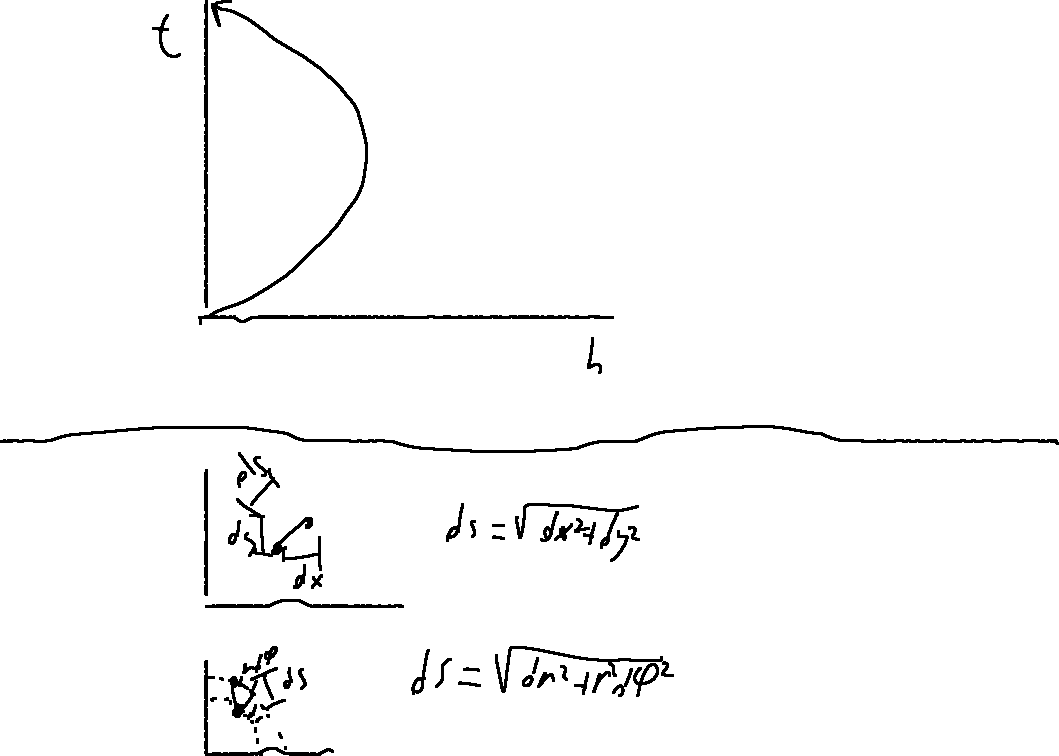
\includegraphics[width=10cm]{1-07-1.png}
	\caption*{Euclidean Geometries}
\end{figure*}
If we now seek to calculate the circumference of a circle using these two different coordinate systems:
\begin{align*}
	C &= \int ds \\
	C &= \int \sqrt{dx^2 + dy^2} \\
	C &= 2\int_-R^R \sqrt{1 + y'\ ^2}dx \\
	C &= 2R\int_-1^1 \frac{dv}{\sqrt{1-v^2}} \\
	C &= 2\pi R
\end{align*}
In the case of polar coordinates though:
\begin{align*}
	C &= \int ds \\
	C &= \int_0^{2\pi} R d\phi \\
	C &= 2\pi R
\end{align*}

We can see that both of these describe Euclidean geometries, but if we move to the Geometry on the surface of a sphere:

The line element is:
\begin{align*}
	ds^2 &= a^2 d\theta^2 + a^2\sin^2\theta d\phi^2
\end{align*}
We can w.l.o.g rotate our sphere such that our circle is moving along a curve where $\theta$ is constant. Therefore we have:
\begin{align*}
	ds &= a\sin\theta d\phi \\
	C &= a2\pi \sin\theta
\end{align*}
If instead we have a circle of radius r, on a sphere of radius a, we choose coordinates with varying $\theta$ but constant $\phi$, so:
\begin{align*}
	ds &= ad\theta \\
	r &= \int ds \\
	r &= \int _0^\theta ad\theta \\
	r &= a\theta \\
	C &= 2\pi a \sin \frac{r}{a}
\end{align*}
Which matches Euclidean geometry in the small r limit.

In GR we will often take a line element and try to use it to understand the underlying geometry. For example we consider $ds^2 = a^2(d\theta^2 f^2(\theta) d\phi^2)$. If we choose $\theta = \sin\theta$ then we are working on the surface of a sphere.
The first property we can not is that the line element is unchanged with $\phi$, so this must have a symetry around the z axis. If we look at $f(\theta) = \sin\theta(1-\frac{3}{4}\sin^2\theta)$, we end up with a peanut geometry.
\begin{figure*}[h]
	\centering
	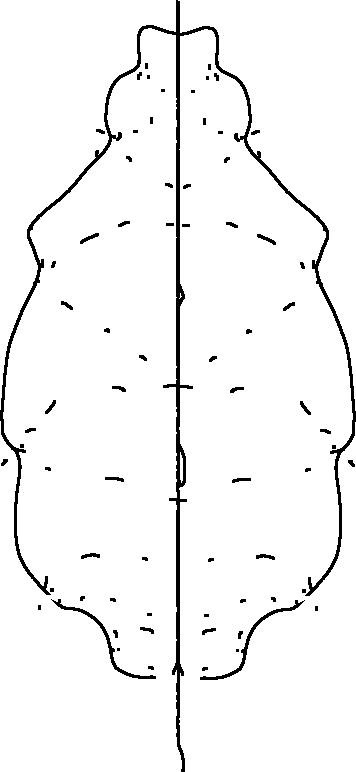
\includegraphics[width=10cm]{1-07-2.png}
	\caption*{Our general $f(\theta)$ geometry}
\end{figure*}

In an inertial frame an observer will have a set of coordinates $t$ such that $\frac{d^2x_i}{dt^2}=0$. A pair of inertial frames can differ by constant displacements, uniform velocities, and constant rotations.

Looking at a pair of frames that only differ by displacements $(x,y,z)$, $(x',y',z')$, if we have this displacement be $d$ along the x axis we know:
\begin{align*}
	x' &= x-d & y'&= y & z' &= z
\end{align*}
Instead for a rotation $\theta$ about the z axis:
\begin{align*}
	x' &= \sin\theta y + \cos\theta x &
	y' &= \cos\theta y - \sin \theta x &
	z' &= z
\end{align*}
If we inestead have a uniform velocity about the x axis, we instead have:
\begin{align*}
	x' &= x -vt' &
	y' &= y &
	z' &= z
\end{align*}

For a point mass experience a gravitational attraction we see:
\begin{align*}
	\bm{F} &= -\frac{GmM}{r^2} \hat{e}_r \\
	\Phi(\bm{x}) &= -\frac{GM}{r} \\
	\Phi(\bm{x}) &= -\frac{GM}{|\bm{x} - \bm{x}_A|}
\end{align*}
If we add multiple point masses:
\begin{align*}
	\Phi(\bm{x}) &= \sum_A-\frac{GM_A}{|\bm{x} - \bm{x}_A|}
\end{align*}
Taking the continuum limit:
\begin{align*}
	\Phi(\bm{x}) &= -\int d^3x' \frac{G\mu(\bm{x}')}{|\bm{x} - \bm{x}'|}
\end{align*}
Which gives rise to the gravitational field:
\begin{align*}
	\bm{g}(\bm{x}) &= -\del\Phi(\bm{x})
\end{align*}
From which we can take a differential form of our potential:
\begin{align*}
	\del\cdot\bm{g} &= -4\pi G\mu(\bm{x}) \\
	\del^2\Phi(\bm{x}) &= -4\pi G\mu(\bm{x}) \\
	m\bm{a} &= -m\del\Phi \\
	\bm{a} &= -\del\Phi
\end{align*}
Where we note that in Newtonian gravity the fact that gravitational mass and the inertial mass being equivalent seems to be a coincidence.


\subsection{Varational Principle}
If we have 1 dimensional motion of a particle with mass $m$ in a potential $V(x)$, then we can define a Lagrangian:
\begin{align*}
	\mathcal{L}(x,\dot{x}) &= \frac{m}{2}\dot{x}^2  - V(x)
\end{align*}
From which we can say:
\begin{align*}
	\frac{d}{dt} \partder{\mathcal{L}}{\dot{x}} &= \partder{\mathcal{L}}{x} \\
	m\ddot{x} &= -\frac{dV}{dx}
\end{align*}
We can also talk about our action $S = \int dt \mathcal{L}(\dot{x},x)$ which is a functional acting on our paths.
In Newtonian mechanics we can define our varaitional principle as: of all curves connecting $x_a,t_a$ to $x_b,t_b$, then the paths that extrimize the action satisfy Lagrange's equation.

The extrema of $f(x,x^2,\ldots,x^n)$ is where all partial derivitives $\partial_x^a f$ vanish, in other words:
\begin{align*}
	\delta f  &= \sum_a \partial_x^a f \delta x^a = 0
\end{align*}
We would now like to compute the variation of our action:
\begin{align*}
	\delta S[x(t)] &= \int dt \left[\partder{\mathcal{L}}{\dot{x}} \delta \dot{x} + \partder{\mathcal{L}}{x}\delta x\right] \\
	\delta S[x(t)] &= \int dt \left[- \frac{d}{dt}\partder{\mathcal{L}}{\dot{x}} + \partder{\mathcal{L}}{x}\right]\delta x
\end{align*}

\section{Special Relativity}
The speed of light is initially derived from Maxwell's equations. Initially it was theorized that there was an ``ether'' in which the speed of light was a constant, because under Galilean relativity velocities would change without an ether.
The Michaelson-Morely experiment disproved the notion of an ether, and lead to the formation of special relativity.

\subsection{Simultaneous events}
In Galilean relativity/Newtonian mechanics it is clear that you can label whether or not events are simultaneous.

We now move to labeling events in spacetime $(t,x,y,z)$.

For any worldline we can restrict the slope to be less than or equal to 1 because:
\begin{align*}
	\frac{d (ct)}{dx} &= \frac{c}{v_x} \leq 1
\end{align*}

\begin{figure*}[h]
	\centering
	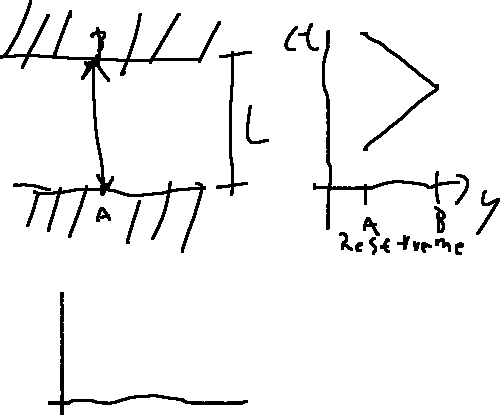
\includegraphics[width=10cm]{1-09-1.png}
	\caption*{Diagram of worldlines for the mirrors}
\end{figure*}
In an inertial frame if we consider two mirrors, then we see the round trip time will be $\Delta t = \frac{2L}{c}$. We can alos condsider this in a boosted frame, moving at a velocity $v$ in parallel to the surface of the mirrors, we see:
\begin{align*}
	\Delta x' &= v \Delta t' \\
	D &= 2\sqrt{L^2 + \left(\frac{\Delta x'}{2}\right)^2} \\
	\Delta t' &= \frac{2}{c}\sqrt{L^2 + \left(\frac{\Delta x'}{2}\right)^2}
\end{align*}

If we now consider the quantity $-(c\Delta t)^2 + (\delta \bm{r})^2$ in each coordinate system. In the boosted frame:
\begin{align*}
	-(c\Delta t')^2 + (\Delta x')^2 &= -4 (L^2 + \frac{\Delta x'\ ^2}{4}) + \Delta x'\ ^2 \\
	-(c\Delta t')^2 + (\Delta x')^2 &= -4 L^2 \\
	-(c\Delta t')^2 + (\Delta x')^2 &= -(c\Delta t)^2
\end{align*}
So it is the same in both frames.

This introduces the principle of relativity which say that our line element that defines distince have the same form in all inertial frames. In flat spacetime this line element is the one chosen above:
\begin{align*}
	ds^2 = -(c dt)^2 + dx^2 + dy^2 + dz^2
\end{align*}
Which we refer to as Minkowski space/the Minkowski line element.

From now on lowercase letters refer to spacetime, and uppercase letters refer to just space.

We say that particles with mass move along time-like world lines.

To measure distance along the worldline we'll use a ``proper time'' $\tau$ where $d\tau^2 = -\frac{ds^2}{c^2}$. We can say that two events are spacelike seperated if $(\Delta s)^2 >0$, timelike seperated if $(\Delta s)^2 <0$, and null for $(\Delta s)^2 =0$.

\subsection{Lorentz Boosts}
We will soon start dropping the factors of $c$ in many equations accepting the convention that $c=1$. 
In order to handle changing frames with a constant velocity between them, we need to use what's known as the Lorentz boost to transform instead of our simple Galilean boost.
This transformation will mix spatial and temporal dimensions in a manner somewhat analagous to rotations in Euclidean geometry:
\begin{align*}
	ct' &= \cosh\theta ct - \sinh\theta x \\
	x' &= -\sinh\theta ct + \cosh\theta x \\
	y' &= y \\
	z' &=z
\end{align*}
If we look at a worldline of a stationary particle in the boosted frame, we can see it corresponds to a constant velocity of $c\tanh\theta$ in the unboosted frame. Since $\cosh^2\theta -\sinh^2\theta = 1$ we can see:
\begin{align*}
	t' &= \gamma\left(t - \frac{vx}{c^2}\right) \\
	x' &= \gamma\left(x - v t\right) \\
	y' &= y \\
	z' &= z
\end{align*}
If we take the small velocity limit $v \ll c$, then:
\begin{align*}
	t' &= t \\
	x' &= x - v t \\
	y' &= y \\
	z' &= z
\end{align*}

We will now additionally add the conventions that we will use throughout the class. 
We will use the zeroeth index to refer to time throughtout the class, and will additionally use the einstein summation notation, i.e. $a^\alpha \hat{e}_\alpha = \sum_\alpha a^\alpha \hat{e}_\alpha$. 
We will also use greek indicies for all 4 spacetime coordinates, and latin indicies for only the spatial components.

The Lorentz boost of a vecotr is:
\begin{align*}
	a^t\ ' &= \gamma(a^t - va^x) \\
	a^x\ ' &= \gamma(a^x - va^t) \\
	a^y\ ' &= a^y \\
	a^z\ ' &= a^z
\end{align*}
And a scalar product is defined:
\begin{align*}
	\bm{a}\cdot\bm{b} &= (a^\alpha b^\beta) (\hat{e}_\alpha\cdot \hat{e}_\beta) \\
	\bm{a}\cdot\bm{b} &= (a^\alpha b^\beta) \eta_{\alpha\beta}
\end{align*}
Where for minkowski space:
\begin{align*}
	\eta_{\alpha\beta} &= \begin{pmatrix}
		-1 & 0 & 0 & 0 \\
		0 & 1 & 0 & 0 \\
		0 & 0 & 1 & 0 \\
		0 & 0 & 0 & 1
			      \end{pmatrix}
\end{align*}
So in flat space:
\begin{align*}
	\bm{a}\cdot\bm{b} &= -a^tb^t + a^x b^x + a^y b^y + a^z b^z
\end{align*}

When talking about worldilines we will typically refer to the position as a function of proper time, and a four velocity $u^\alpha = \frac{d x^\alpha}{d\tau}$. This can be written in terms of the three velocity:
\begin{align*}
	u^t &= \frac{dt}{d\tau} \\
	u^t &= \frac{1}{\sqrt{1-v^2}} \\
	u^i &= \frac{dx^i}{d\tau} \\
	u^i &= \frac{v^i}{\sqrt{1-v^2}} \\
	u^\alpha &= (\gamma,\gamma v^i)
\end{align*}

If we now compute the magnitude of $u^\alpha$, i.e. $u_\alpha u^\alpha = -1$

\subsection{Dynamics}
In the abscencce of outside forces, we should have constant 4 velocities, so (in any inertial frame):
\begin{align*}
	\frac{d u^\alpha}{d\tau} &= 0
\end{align*}
If we have a force applied though we see:
\begin{align*}
	m\frac{d u^\alpha}{d\tau} &= f^\alpha
\end{align*}
We say this is a 4 acceleration $a^\alpha = \frac{d u^\alpha}{d\tau}$, so we have $f^\alpha = m a^\alpha$.
We additionally say we have a 4 momentum $p^\alpha = m u^\alpha$, where clearly $p^\alpha p_\alpha = -m^2$.
If we look at our 4 momentum in terms of it's components in flat space:
\begin{align*}
	p^t &= \frac{m}{\sqrt{1-v^2}} \\
	p^i &= \frac{mv^i}{\sqrt{1-v^2}}
\end{align*}
In a low velocity limit we see:
\begin{align*}
	p^t &\approx m + \frac{m}{2}v^2 \\
	p^i &= m v^i
\end{align*}
So we can say (if we include a constant ress mass energy) $p^\alpha = (E,p^i)$


We know that in special relativity we must have our velocities sum in such a way that the velocity of light will not change, but the velocity of slower objects will (and in the non-relativistic limit they simply add).
We can say:
\begin{align*}
	dt' &= \gamma(dt - vdx) \\
	dx' &= \gamma(dx -v dt) \\
	\frac{dx'}{dt'} &= \frac{\frac{dx}{dt} - v}{1 -v \frac{dx}{dt}}
\end{align*}
If we choose $\frac{dx}{dt} = 1$ then $\frac{dx'}{dt'} = 1$. So this works for light like velocities how we want it to.

\subsection{Four vectors and coordinate systems}
We can write our line element in terms of our metric:
\begin{align*}
	ds^2 &= \eta_{\alpha\beta} dx^\alpha dx^\beta
\end{align*}
We tend to paramterize paths in terms of the proper time of the particle while moving. So our four velocity in terms of the proper time is then:
\begin{align*}
	u^\alpha &= \frac{dx^\alpha}{d\tau}
\end{align*}
Our temporal component is then going to be $u^t = \gamma$ and our spatial components are $u^i = \gamma v^i$, so we cam say our four velocity is then $u^\mu = (\gamma,\gamma \bm{V}$
\subsection{Dynamics}
We now consider Newton's first law in special relativity:
\begin{align*}
	\frac{d u^\mu}{d\tau} &= 0
\end{align*}
In the abscence of forces. In order to posit Newton's second law, we want it to abey this in the abscence of forces, be properly relativistic, and reduce to the classical result in the non-relativistic limit:
\begin{align*}
	m\frac{du^\mu}{d\tau} &= f^\mu
\end{align*}
Which since this is a 4-vector equation obviously obeys relativity, and it clearly obeys the first law when $f^\mu =0$. In order to check the classical limit, we define the four acceloration $a^\mu = \frac{du^\mu}{d\tau}$.
This gives us the classic $f^\mu = m a^\mu$. This is a set of 4 equations, which is one more than our classical set of equations. This is of course constrained by our restriction on the length of $u$, $u^\mu u_\mu = -1$, so:
\begin{align*}
	m \frac{d}{d\tau} u^\mu u_\mu &= 0 \\
	u^\mu a_\mu &= 0 \\
	f_\mu u^\mu &=0
\end{align*}
We now look at energy and momentum.
\begin{align*}
	p^\mu &= m u^\mu \\
	\frac{dp^\mu}{d\tau} &= f^\mu \\p^\mu p_\mu &= -m^2 \\
	p^t &= \frac{m}{1-v^2} \\
	p^i &= \frac{mv^i}{\sqrt{1-v^2}}
\end{align*}
If we take the limit where $v\ll 1$:
\begin{align*}
	p^t &= m + \frac{1}{2} mv^2 \\
	p^i &= mv^i
\end{align*}
So we say $p^\mu = (E, P)$

We now look to extract our spatial forces from our 4 force. We define this by $F^i = \frac{dP^i}{dt}$, so:
\begin{align*}
	f^i &= \frac{dP^i}{d\tau} \\
	f^i &= \gamma F^i
\end{align*}
We also know:
\begin{align*}
	f^t u^t &= f_i u^i \\
	f_t\gamma &= \gamma^2 F_i V^i \\
	f^t &= \gamma F_i V^i \\
	f^\mu &= (\gamma F_i V^i, \gamma F^i)
\end{align*}
\section{Curved Spacetime}
We say that our line element:
\begin{align*}
	ds^2 &= -dt^2 + dx^2 + dy^2 + dz^2
\end{align*}
Can be used to find line elements in other coordinate systems, such as with spherical coordinates. Here we will have:
\begin{align*}
	ds^2 &= -dt^2 + dr^2 + r^2 d\theta^2 + r^2\sin^2\theta d\phi^2
\end{align*}
This introduces a coordinate singularity, as if you choose $\theta=0$ all values for $\phi$ are mapped to the same point. This is non-physical though as it doesn't appear in caresian coordinates.

Let us now consider 2-D polar coordinates in flat space:
\begin{align*}
	dS^2 &= dr^2 = r^2d\phi^2
\end{align*}
If we transform to $r = \frac{a^2}{r'}$:
\begin{align*}
	dS^2 &= \frac{a^4}{r'\ ^4} (dr'\ ^2 + r'\ ^2 d\phi^2)
\end{align*}
Which has an infinite line element at $r' = 0$, but this makes sense as our transformation only gives us $r' = 0$ if $r = \infty$.
\subsection{Penrose diagrams}
We begin with our line element for flat spacetime in spherical coordinates:
\begin{align*}
	ds^2 &= -dt^2 + dr^2 + r^2 d\theta^2 + r^2\sin^2\theta d\phi^2
\end{align*}
We now define a coordinate $u = t - r$ and $v = t + r$, then we see we have a new line element:
\begin{align*}
	ds^2 &= -dudv + \frac{1}{4} (u-v)^2 (d\theta^2 \sin^2\theta d\phi^2)
\end{align*}
This implies off diagonal metric elements. In this coordinate system, lines of constant $u$ and $v$ are light paths.

We now make one more transformation:
\begin{align*}
	u' &= \arctan u &
	u' &= \frac{t' - r'}{2} \\
	v' &= \arctan{v} &
	v' &= \frac{t' + r'}{2}
\end{align*}
This will map all $(t,r)$ to $r' > 0$, $v' < \frac{\pi}{2}$, $u' > -\frac{\pi}{2}$
\begin{figure*}[h]
	\centering
	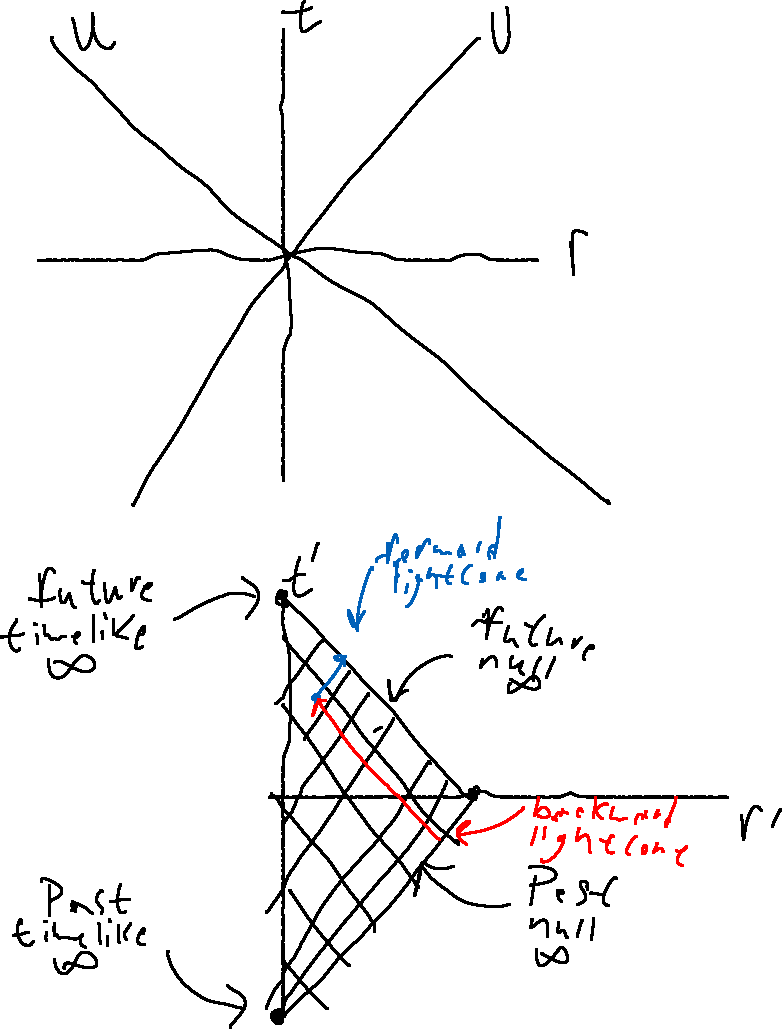
\includegraphics[width=6cm]{1-14-1.png}
	\caption*{Penrose Diagrams}
\end{figure*}
\subsection{Local Inertial frames}
We say that the equivalence priciple states that in local coordinates it is impossible to determine whether or not you are in curved spacetime.

In general we refer to our metric as $g_{\alpha\beta}$. Given some general metric (as a function of spacetime) $g_{\alpha\beta}(\bm{x})$, at every point $P$ we can invent a new coordinate system where:
\begin{align*}
	g_{\alpha\beta}'(x'_P) &= \eta_{\alpha\beta} \\
	\partder{g_{\alpha\beta}}{x'}|_P &= 0
\end{align*}
Which defines a local inertial frame at $p$.

Just as before we have the following types of distance:
\begin{align*}
	ds^2 < 0 & \text{timelike} \\
	ds^2 &= 0 & \text{null/lightlike} \\
	ds^2 >0 & \text{spacelike}
\end{align*}
Where our proper time can be defined as:
\begin{align*}
	\tau_{AB} &= \int_A^B \sqrt{-g_{\alpha\beta}(x)dx^\alpha dx^\beta}
\end{align*}
\subsection{Length, area, volume, and 4-volume}
For now we consider:
\begin{align*}
	ds^2 &= g_{00} (dx^0)^2 + g_{11}(dx^1)^2 + g_{22} (dx^2)^2 + g_33(dx^3)^2
\end{align*}
Therefore our area can be expressed as (for a rectangle in $x^1$, $x^2$):
\begin{align*}
	dA &= \sqrt{g_{11} g_{22}} dx^1 dx^2
\end{align*}
And for our three volume:
\begin{align*}
	dV &= \sqrt{g_{11}g_{22}g_{33}} dx^1 dx^2 dx^3 
\end{align*}
and finally four volume:
\begin{align*}
	dv &= \sqrt{-g_{00}g_{11}g_{22} g_{33}}dx^0dx^1dx^2dx^3
\end{align*}
If we let $g$ denote $\det g_{\alpha\beta}$ then:
\begin{align*}
	dv &= \sqrt{g} d^4 x
\end{align*}

We now consider the line element:
\begin{align*}
	dS^2 &= \frac{dr^2}{1-\left(\frac{r}{a}\right)^2} + r^2(d\theta^2 + \sin^2\theta d\phi^2)
\end{align*}
If we look at $r=R$ and $\theta = \frac{\pi}{2}$ then we calculate our circuference:
\begin{align*}
	C &= \oint dS \\
	C &= 2\pi R
\end{align*}
And then the distance from the center to the surface alone a line of constant $\theta$ and $\phi$:
\begin{align*}
	S &= \int dS \\
	S &= a\arcsin \frac{R}{a}
\end{align*}
Looking at the area of our surface at constant radius we find:
\begin{align*}
	A &= \int dA \\
	A &= 4\pi R^2
\end{align*}
And we finally consider the volume inside a radius $R$:
\begin{align*}
	V &= \int dV \\
	V &= \int_0^R dr\in_0^\pi d\theta\int_0^{2\pi}d\phi \frac{r^2\sin\theta}{1-\left(\frac{r}{a}\right)^2} \\
	V &= 4\pi a^3 \left(\frac{1}{2}\arcsin\left[\frac{R}{a}  - \frac{R}{2a} \sqrt{1 - \left(\frac{R}{a}\right)^2}\right]\right)
\end{align*}

\subsection{Embedding Diagrams}
We consider the line element:
\begin{align*}
	ds^2 &= -dt^2 + dr^2 +(b^2 + r^2)(d\theta^2 + \sin^2\theta d\phi^2)
\end{align*}
(Note we call this a static metric since there is no explicit time dependance). This is flat when $b=0$ but is not flat otherwise.

We now consider a slice where $t$ is constant:
\begin{align*}
	dS^2 &= dr^2 +(b^2 + r^2)(d\theta^2 + \sin^2\theta d\phi^2)
\end{align*}
And now constant angle ($\theta = \frac{\pi}{2}$:
\begin{align*}
	d\Sigma^2 &= dr^2 +(b^2 + r^2)d\phi^2
\end{align*}
We now consider this in cylindrical coordinates in flat space:
\begin{align*}
	dS^2 &= d\rho^2 + \rho^2 d\psi^2 + dz^2
\end{align*}
We look at this in terms of $z= z(r)$, $\rho = \rho(r)$ and $\psi = \phi$
We then have:
\begin{align*}
	d\psi &= d\phi \\
	dz &= \frac{dz}{dr} dr \\
	d\rho &= \frac{d\rho}{dr} dr
\end{align*}
So then:
\begin{align*}
	d\Sigma^2 &= \left(\frac{d\rho}{dr}\right)^2 dr^2 + \rho^2d\phi^2 + \left(\frac{dz}{dr}\right)^2 dr^2 \\
	d\Sigma^2 &= \left[\left(\frac{d\rho}{dr}+ \left(\frac{dz}{dr}\right)^2 \right)^2\right] dr^2 + \rho^2d\phi^2
\end{align*}
So then by inspection:
\begin{align*}
	\rho^2 &= r^2 + b^2 \\
	\left(\frac{dz}{dr}\right)^2 + \left(\frac{d\rho}{dr}\right)^2 &= 1 \\
	\left(\frac{d\rho}{dr}\right)^2 &= \frac{r^2}{\rho^2} \\
	\left(\frac{d\rho}{dr}\right)^2 &= \frac{r^2}{r^2 + b^2} \\
	\left(\frac{dz}{dr}\right)^2 &= \frac{1}{1 + \left(\frac{r}{b}\right)^2} \\
	z &= b\text{arcsinh}\frac{r}{b}
\end{align*}


Rewriting this in terms of $\rho$ we find:
\begin{align*}
	\sinh\frac{z}{b} &= \sqrt{\left(\frac{\rho}{b}\right)^2 - 1} \\
	\sinh^2\frac{z}{b} &= \left(\frac{\rho}{b}\right)^2 - 1 \\
	\frac{\rho}{b} &= \cosh \frac{z}{b}
\end{align*}
\begin{figure*}[h]
	\centering
	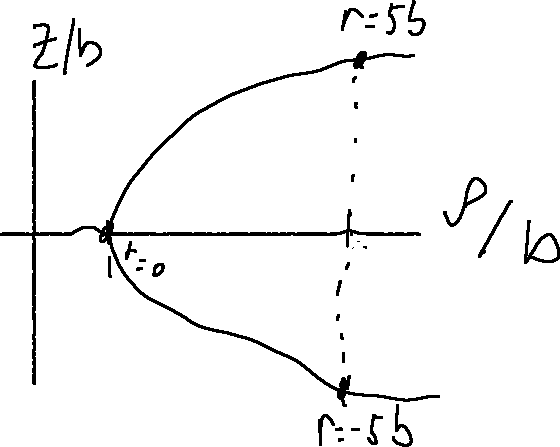
\includegraphics[width=6cm]{1-16-1.png}
	\caption*{Our embedding diagram}
\end{figure*}
Passing through $r=0$ here refers to moving to a distinct region of spacetime that is still flat but not the region of spacetime that we reached in the positive direction.
\subsection{Vectors in curved spacetime}
First we say that a vector is defined at a point in spacetime. Vector fields are generally functions of spacetime:
\begin{align*}
	\bm{a} &= \bm{a}(x^\mu)
\end{align*}
We now extend our basis vectors to be vector fields that are position dependant, i.e.:
\begin{align*}
	\bm{a} &= a^\alpha(x^\mu) \bm{e}_\alpha(x^\mu)
\end{align*}
So our dot product becomes:
\begin{align*}
	\bm{a}\cdot\bm{b} &= (\bm{e}_\alpha\cdot\bm{e}_\beta)a^\alpha b^\beta
\end{align*}
If we define a locally flat frame we conventionallly write: $\bm{e}_{\hat{\alpha}} \cdot\bm{e}_{\hat{\beta}} = \eta_{\hat{\alpha}\hat{\beta}}$.
These locally flat frames describe how an observer would view things. We do that by saying $\bm{e}_{\hat{t}} = \bm{u}_\text{obs}$.

Additionally we will have a coordinate basis where:
\begin{align*}
	u^\alpha &= \frac{dx^\alpha}{d\tau}
\end{align*}
Which in general will not be the same as our locally flat or orthonormal basis. We know that:
\begin{align*}
	\bm{u}\cdot\bm{u} &= -1 \\
	ds^2 &= g_{\alpha\beta}dx^\alpha dx^\beta \\
	ds^2 &= -d\tau^2
\end{align*}
We say we can write:
\begin{align*}
	g_{\alpha\beta}u^\alpha u^\beta &= -1
\end{align*}
In the coordinate basis.

To define the coordinate basis we say it is the basis in which:
\begin{align*}
	\bm{e}_\alpha(x^\mu)\cdot\bm{e}_\beta(x^\mu) &= g_{\alpha\beta}(x^\mu)
\end{align*}

So in summary we use our coordinate basis to do calculations, while we use orthonormal/locally flat basis to do interpretations. We will also use $\hat{\alpha}$ to refer to our orthonormal basis.

We now consider a coordinate basis and an orthonormal basis:
\begin{align*}
	\bm{a} &= a^\alpha\bm{e}_\alpha \\
	\bm{a} &= a^{\hat{\alpha}}\bm{e}_{\hat{\alpha}}
\end{align*}
In order to transform between these we need to express the components in terms of the other set of basis vectors, i.e:
\begin{align*}
	a^\alpha &= a^{\hat{\beta}}(\bm{e}_{\hat{\beta}})^\alpha \\
	a^{\hat{\alpha}} &= a^{\beta}(\bm{e}_{\beta})^{\hat{\alpha}}
\end{align*}
\subsection{Geodesics}
THe worldline of a free test particle between two timelike seperated points will exteremize the proper time between them. These extermized paths are known as geodesics, and the equations of motion that determine them are known as the geodesic equations.

For example we consider the equations for geodesics in plane in polar coordinates.
\begin{align*}
	dS^2 &= dr^2 + r^2 d\phi^2
\end{align*}
We describe a curve betwweeen two points $A$ and $B$ parametrically as $r(\sigma)$ and $\phi(\sigma)$, where $\sigma\in[0,1]$:
\begin{align*}
	S_{AB} &= \int_A^B dS \\
	S_{AB} &= \int_0^1 d\sigma \sqrt{\left(\frac{dr}{d\sigma}\right)^2 + r^2 \left(\frac{d\phi}{d\sigma}\right)^2}
\end{align*}
We can see that this defines a lagrangian:
\begin{align*}
	\mathcal{L}&= \sqrt{\left(\frac{dr}{d\sigma}\right)^2 + r^2 \left(\frac{d\phi}{d\sigma}\right)^2} \\
	\frac{d}{d\sigma} \left(\frac{1}{\mathcal{L}} \frac{dr}{d\sigma}\right) &= \frac{r}{\mathcal{L}} \left(\frac{d\phi}{d\sigma}\right)^2 \\
	\frac{d^2r}{ds^2} &= r\left(\frac{d\phi}{ds}\right)^2
\end{align*}

The equations for time-lke geodesics will be talked about in terms of proper time:
\begin{align*}
	\tau_{AB} &= \int_A^Bd\tau \\
	\tau_{AB} &= \int_A^B\sqrt{-g_{\alpha\beta}(x) dx^\alpha dx^\beta} \\
	\tau_{AB} &= \int_0^1d\sigma\sqrt{-g_{\alpha\beta}(x) \frac{dx^\alpha}{d\sigma} \frac{dx^\beta}{d\sigma}}
\end{align*}
Which gives us a Lagrangian:
\begin{align*}
	\mathcal{L} &= \sqrt{-g_{\alpha\beta}(x)\frac{dx^\alpha}{d\sigma}\frac{dx^\beta}{d\sigma}}
\end{align*}
Where:
\begin{align*}
	\partder{\mathcal{L}}{dx^\alpha} &= \frac{d}{d\sigma} \partder{\mathcal{L}}{\frac{dx^\alpha}{d\sigma}}
\end{align*}

We now return to our wormhole geometry:
\begin{align*}
	ds^2 &= -dt^2 + dr^2 + (r^2 + b^2)(d\theta^2 + \sin^2\theta d\phi^2) \\
	\mathcal{L} &= \sqrt{\left(\frac{dt}{d\sigma}\right)^2 - \left(\frac{dr}{d\sigma}\right)^2 0 (b^2 + r^2)\left[\left(\frac{d\theta}{d\sigma}\right)^2 + \sin^2\theta \left(\frac{d\phi}{d\sigma}\right)^2\right]}
\end{align*}
We note that $\partder{\mathcal{L}}{()} \propto \frac{1}{\mathcal{L}}$ and we also see:
\begin{align*}
	\mathcal{L} &= \frac{d\tau}{d\sigma} \\
	\partder{\mathcal{L}}{t} &= 9 &
	\frac{d^2 t}{d\tau^2} &= 0 \\
	\partder{\mathcal{L}}{r} &= -\mathcal{L}r\left[\left(\frac{d\theta}{d\sigma}\right)^2 + \sin^2\theta \left(\frac{d\phi}{d\sigma}\right)^2\right] \\
	\partder{\mathcal{L}}{\frac{dr}{d\sigma}} &= -\frac{d r}{d\tau}
\end{align*}
WHich then implies:
\begin{align*}
	\frac{d^2 r}{d\tau^2} &= r\left[\left(\frac{d\theta}{d\sigma}\right)^2 + \sin^2\theta \left(\frac{d\phi}{d\sigma}\right)^2\right] \\
\end{align*}
We now look at the rest of the problem:
\begin{align*}
	\frac{d}{d\tau} \left[(b^2 + r^2)\frac{d\theta}{d\tau}\right] &= (b^2 + r^2)\sin\theta\cos\theta\left(\frac{d\theta}{d\tau}\right)^2 \\
	\frac{d}{d\tau} \left[(b^2+ r^2)\sin^2\theta \frac{d\phi}{d\tau}\right] &= 0
\end{align*}

The general form of the geodesic equation for timelike geodesics will be:
\begin{align*}
	\frac{d^2x^\alpha}{d\tau^2} &= -\Gamma_{\beta\gamma}^\alpha \frac{dx^\beta}{d\tau} \frac{dx^\gamma}{d\tau}
\end{align*}
This is a set of for equations, one for each $\alpha$. The $\Gamma$ symbols are called the Christoffel symbols, are constructed from our metric and 1st derivitives, and are notably not tensors:
\begin{align*}
	u^z\alpha &= \frac{dx^\alpha}{d\tau} \\
	\frac{du^\alpha}{d\tau} &= -\Gamma_{\beta\gamma}^\alpha u^\beta u^\gamma
\end{align*}
These are symmetric in the lower indicies.
`
Looking back at the plane in polar coordinates:
\begin{align*}
	\frac{d^2 r}{dS^2} &= r \left(\frac{d\phi}{dS}\right)^2 &
	\frac{d}{dS} \left(r^2 \frac{d\phi}{dS} \right) &= 0 \\
	\Gamma_{\phi\phi}^r &= -r &
	\Gamma_{r\phi}^\phi &= \frac{1}{r}
\end{align*}
Where all the others will be 0.

We can additionally compute the Chrisoffel symbols via:
\begin{align*}
	g_{\alpha\delta}\Gamma_{\beta\gamma}^\delta &= \frac{1}{2}\left(\partder{g_{\alpha\beta}}{x^\gamma} + \partder{g_{\alpha\gamma}}{x^\beta} - \partder{g_{\beta\gamma}}{x^\alpha}\right)
\end{align*}


We now look to compute the travel time through a wormhole geometry as an example. We have our traveler begin at a coordinate radius $R$ and allow them to fall inward through the Wormhole.
Therefore we say:
\begin{align*}
	u^r &= U
\end{align*}
So we have an initial radial 4-velocity. We now attempt to compute the time the traveler experiences traveling to $r=-R$. In order to have the total length of our 4-velocity equal to $-1$ we say:
\begin{align*}
	\bm{u} &= (\sqrt{1+ U^2},U,0,0)
\end{align*}
We can see from our prior work in this geometry:
\begin{align*}
	\partder{u^r}{\tau} &= 0
\end{align*}
So moving along the radius we see that the radial component is constant and therefore we can say:
\begin{align*}
	r(\tau) &= U\tau \\
	\Delta\tau &= \frac{2R}{U}
\end{align*}
Recall from mechanics, that conservation laws give first integrals of EOM, which generally reduce the number of equations we need to solve.
In GR we know that the four velocity's length is always conserved $g_{\alpha\beta} u^\alpha u^\beta = -1$.
Symmetries in our spacetime will give us other conservation laws. From Newtonian mechanics we know that energy conservation arises from a potential that is invariant under time translation.
Conserved linear momentum arrises from translation invariance. For angular momentum we see a conservation law will arise from rotational invariance (spherical symmetry).

In GR we look at symmetries in spacetime. These occur when the metric is invariant under displacements in a given coordinate.
The four vector $\xi = (0,1,0,0)$ which captures our symmetry is called the Killing vector associated with the symmetry.

For example in flat space:
\begin{align*}
	dS^2 &= dx^2 + dy^2 + dz^2
\end{align*}
We can immediately see that we have killing vectors $(1,0,0)$, $(0,1,0)$, and $(0,0,1)$. We can see if we change coordinate to spherical coordinates we have:
\begin{align*}
	dS^2 &= dr^2 + r^2 d\theta^2 + r^2\sin^2\theta d\phi^2
\end{align*}
So we can see we have the killing vector $(0,0,1)$.

These killing vectors are associated with constants of motion: 
\begin{align*}
	\bm{\xi}\cdot\bm{u} &= \text{const}
\end{align*}
If our metric (and therefore our Lagrangian) are independant of some coordinate $x^1$, then:
\begin{align*}
	\partder{\mathcal{L}}{x^1} &=0 \\
	\frac{d}{d\sigma} \partder{\mathcal{L}}{\frac{dx^1}{d\sigma}} &= 0 \\
	\partder{\mathcal{L}}{\frac{dx^1}{d\sigma}} &= -g_{1\beta} \frac{1}{\mathcal{L}} \frac{dx^\beta}{d\sigma} \\
	\partder{\mathcal{L}}{\frac{dx^1}{d\sigma}} &= -g_{1\beta} \frac{dx^\beta}{d\tau} \\
	\partder{\mathcal{L}}{\frac{dx^1}{d\sigma}} &= -g_{\alpha\beta} \xi^\alpha\frac{dx^\beta}{d\tau} \\
	\partder{\mathcal{L}}{\frac{dx^1}{d\sigma}} &= -\bm{\xi}\cdot\bm{u}
\end{align*}
Looking now at null geodesics (the paths of photons). We can no longer use proper time to parameterize our paths since photons have $\Delta\tau = 0$. We choose our parameter to be $\lambda$, so:
\begin{align*}
	u^\alpha &= \frac{dx^\alpha}{d\lambda} \\
	\bm{u}\cdot\bm{u} &= g_{\alpha\beta} \frac{dx^\alpha}{d\lambda} \frac{dx^\beta}{d\lambda} \\
	\bm{u}\cdot\bm{u} &= 0
\end{align*}
We know in flat spacetime that:
\begin{align*}
	\frac{d^2x^\alpha}{d\lambda^2} &= 0
\end{align*}
We want to generalize this, and we want to be sure to maintain that: 1. in a local inertial frame our generalization reduces to this, and 2. that this takes the same form in all coordinate systems.

We choose as our generalization:
\begin{align*}
	\frac{d^2x^\alpha}{d\lambda^2} &= -\Gamma^\alpha_{\beta\gamma} \frac{dx^\beta}{d\lambda}\frac{dx^\gamma}{d\lambda}
\end{align*}

\subsection{Shwarzchild geometry}
We consider the geometry outside a spherical star:
\begin{align*}
	ds^2 &= -\left(1 -\frac{2GM}{c^2 r}\right)(cdt)^2 + \left(1- \frac{2GM}{c^2 r}\right)dr^2 + r^2 (d\theta^2 + \sin^2\theta d\phi^2)
\end{align*}
We refer to these coordinates as Schwarzchild coordinates. We can immediately see this is spherically symmetric, and that as $r\to\infty$ this becomes flat spacetime.
Additionally we see there are coordinate singularities at $r=0$ and $r=\frac{2GM}{c^2}$. The singularity at $r=0$ can be ignored for physical reasons, and the other one is because of the choice of coordinates, and can be removed by changing coordinates.
Also note that $r$ is not radial distance, but instead related to the surface area of a sphere of that radius. Also this is time independant. We can write killing vector:
\begin{align*}
	\xi &= (1,0,0,0)
\end{align*}
And the geometry at constant $r$ and $t$:
\begin{align*}
	d\Sigma^2 &= r^2(d\theta^2 + \sin^2\theta d\phi^2)
\end{align*}
Where we find another killing vector:
\begin{align*}
	\eta &= (0,0,0,1)
\end{align*}
We may assume that $M$ is the mass of the star, but we now want to interogate this by taking the non-relativistic limit:
\begin{align*}
	\frac{GM}{c^2 r} \ll 1 \\
	ds^2 &\approx -\left(1 - \frac{2GM}{c^2r}\right)(cdt)^2 + \left(1+ \frac{2GM}{c^2 r}\right)dr^2 + r^2 (d\theta^2 + \sin^2\theta d\phi^2)
\end{align*}
Which is the static weak field metric for the Newtonian gravitational potential

Looking at the Schwarzchild radius $r = \frac{2GM}{c^2}$.

Now we look at the effect on light of killing vectors moving away from the singularity of a shwarzchild geometry.
If we have an emission event at fixed radius R emitting a light signal with frequency $\omega_*$ and an infinitely distant observer sees it with frequence $\omega_\infty$.
We know the energy of this photon is $E=\hbar\omega$. And we have a symmetry related to this:
\begin{align*}
	\xi &= (1,0,0,0) \\
	\bm{\xi}\cdot\bm{p} &= \text{const}
\end{align*}
We want to move to orthonormal basis for our observers, in these frames we will have each observers velocity vector be $u = (1,0,0,0)$.

Therefore we say an observer moving with velocity $\bm{u}_\text{obs}$ will measure an energy:
\begin{align*}
	E &= -\bm{p}\cdot\bm{u}_\text{obs} \\
	E &= \hbar\omega
\end{align*}
For any observer we will have four velocity:
\begin{align*}
	\bm{u}_\text{obs}\cdot\bm{u}_\text{obs} &= -1
\end{align*}
In the observers frame:
\begin{align*}
	u_\text{obs}^i &= 0 \\
	g_{tt}(r) u^t_\text{obs}\ ^2 &= -1 \\
	u^t_\text{obs} &= \left(1- \frac{2GM}{c^2 r}\right)^{-\frac{1}{2}}
\end{align*}
So for our stationary observer:
\begin{align*}
	\bm{u}_\text{obs} &= \left(1- \frac{2GM}{c^2 r}\right)^{-\frac{1}{2}}\bm{\xi}
\end{align*}
So:
\begin{align*}
	\hbar\omega_* &= \left(1- \frac{2GM}{c^2 r}\right)^{-\frac{1}{2}}(\bm{\xi}\cdot\bm{p})_R \\
	\hbar\omega_\infty &= (\bm{\xi}\cdot\bm{p})_\infty
\end{align*}
But this is a conserved quantity, so:
\begin{align*}
	(\bm{\xi}\cdot\bm{p})_R &= (\bm{\xi}\cdot\bm{p})_\infty \\
	\omega_\infty &= \omega_* \sqrt{1 - \frac{2GM}{c^2 R}}
\end{align*}


We now look at particle motion in the Schwazchild geometry. We say that the metric will be independant of $t$ and $\phi$. I.e. we have constants:
\begin{align*}
	\bm{\xi}\cdot\bm{u} &= \text{const} &
	\xi &= (1,0,0,0) \\
	\bm{\eta}\cdot\bm{u} &= \text{const} &
	\eta &= (0,0,0,1)
\end{align*}
We say:
\begin{align*}
	e &= -\bm{\xi}\cdot\bm{u} \\
	e &= \left(1- \frac{2M}{r}\right) \frac{dt}{d\tau}
\end{align*}
Which is our conserved energy per unit mass. And we also have:
\begin{align*}
	l &= \bm{\eta}\cdot\bm{u} \\
	l &= r^2\
	sin^2\theta \frac{d\phi}{d\tau}
\end{align*}
Which is our conserved angular momentum per unit mass.

Since the four velocity must be normalized we can say:
\begin{align*}
	\bm{u}\cdot\bm{u} &= -1 \\
	\bm{u}\cdot\bm{u} &= g_{\alpha\beta} u^\alpha u^\beta \\
	\bm{u}\cdot\bm{u} &= -\left(1 - \frac{2M}{r}\right)(u^t)^2 + \left(1 - \frac{2M}{r}\right)^{-1}(u^r)^2 + r^2(u^\phi)^2
\end{align*}
Where we have picked coordinates where we are rotating in the plane $\theta = \frac{\pi}{2}$. Inserting our known constants of motion:
\begin{align*}
	\bm{u}\cdot\bm{u} &= -\left(1 - \frac{2M}{r}\right)e^2 + \left(1 - \frac{2M}{r}\right)^{-1}\left(\frac{dr}{d\tau}\right)^2 + \frac{l^2}{r^2}\\
	\frac{e^2 - 1}{2} &= \frac{1}{2}\left(\frac{dr}{d\tau}\right)^2 + \frac{1}{2}\left[\left(1-\frac{2M}{r}\right)\left(1+ \frac{l^2}{r^2}\right) - 1\right] \\
	\varepsilon &= \frac{e^2 - 1}{2} \\
	\varepsilon &= \frac{1}{2}\left(\frac{dr}{d\tau}\right)^2 + \frac{1}{2}\left[\left(1-\frac{2M}{r}\right)\left(1+ \frac{l^2}{r^2}\right) - 1\right]
\end{align*}
We then define an effective potential:
\begin{align*}
	V_\text{eff} &= \frac{1}{2}\left[\left(1-\frac{2M}{r}\right)\left(1+ \frac{l^2}{r^2}\right) - 1\right] \\
	V_\text{eff} &= -\frac{M}{r} + \frac{l^2}{2r^2} - \frac{Ml^2}{r^3} \\
	\varepsilon &= \frac{1}{2}\left(\frac{dr}{d\tau}\right)^2 + V_\text{eff}(r)
\end{align*}


Now with our effective potential in hand we look for an extrema of the potential:
\begin{align*}
	r_\text{ext} &= \frac{l^2}{2M}\left[1\pm\sqrt{1 - 12\left(\frac{M}{l}\right)^2}\right]
\end{align*}
We now consider what happens to this in some strange conditions. If we set $\frac{l}{M} < \sqrt{12}$, then we see this will have imaginary solutions (which implies the extrema vanish).
Only the larger solution will be stable, so we are more interested in this solution.

\subsection{Radial plunge}
We consider radial freefall from $r=\infty$ starting at rest. Therefore $l = 0$, $u^t = 1$, from our killing vector we know:
\begin{align*}
	e &= \left(1 - \frac{2M}{r}\right)u^t \\
	1 &= \left(1 - \frac{2M}{r}\right)u^t 
\end{align*}
We also know:
\begin{align*}
	\frac{e^2-1}{2} &= \frac{1}{2} u^r\ ^2 - \frac{M}{r} \\
	-\sqrt{\frac{2M}{r}} &= r \\
	\sqrt{r} dr &= -\sqrt{2M} d\tau \\
	u &= \left[ \left(1- \frac{2M}{r}\right)^{-1}, -\sqrt{\frac{2M}{r}}, 0, 0\right] \\
	- \frac{2}{3}r^\frac{3}{2} &= -\sqrt{2M}(\tau_* - \tau) & r(\tau_*) &= 0 \\
	r(\tau) &= \left(\frac{3}{2}\right)^\frac{2}{3} (2M)^\frac{1}{3}(\tau_* - \tau)^\frac{2}{3}
\end{align*}
We now look to find our coordinate time $t$:
\begin{align*}
	e &= \left(1 - \frac{2M}{r}\right)u^t \\
	\frac{dt}{d\tau} &= \left(1 - \frac{2M}{r}\right)^{-1} \\
	\frac{dt}{dr} &= -\left(1 - \frac{2M}{r}\right)^{-1}\left(\frac{2M}{r}\right)^{-\frac{1}{2}} \\
	t &= t_* + 2M\left[ -\frac{2}{3}\left(\frac{r}{2M}\right)^\frac{3}{2} - 2\left(\frac{r}{2M}\right)^\frac{1}{2} + \log|\frac{\sqrt{\frac{r}{2M}} + 1}{\sqrt{\frac{r}{2M}} - 1} |\right]
\end{align*}

\subsection{Stable circular orbits}
We can say that our stable circular orbit ocur with $r=r_\text{ext}$ which decreases with decreasing $\frac{l}{m}$, and we see that the minimum it has is $r_\text{SCO} = 6M$.
We can see that the angular velocities ($\Omega$) in circular orbits (defined relative to a distant observer):
\begin{align*}
	\Omega &= \frac{d\phi}{dt} \\
	\Omega &= \frac{u^\phi}{u^t} \\
	\Omega &= \frac{1}{r^2} \left(1 - 2\frac{M}{r}\right) \frac{l}{e}
\end{align*}
This gives us a relation between $r$ and $l$ using our potential at the minimum, and additionally we see:
\begin{align*}
	e^2 &= \left(1-\frac{2M}{r}\right)\left(1 + \frac{l^2}{r^2}\right) \\
	r_\text{min} &= \frac{l^2}{2M} \left[ 1 + \sqrt{1 - 12\frac{M^2}{l^2}}\right] \\
	\varepsilon &= \frac{1}{2} u^r\ ^2 + V_\text{eff}
\end{align*}
So:
\begin{align*}
	\frac{l}{e} &= \sqrt{Mr} \left(1 - \frac{2M}{r}\right)^{-1} \\
	\Omega^2 &= \frac{M}{r^3}
\end{align*}
Which is Kepler's law!

We now want to look at null trajectories in the Schrwarzchild geometry. We will parameterize this curve using an affine parameter $\lambda$, with the for velocity normalized to $u_\alpha u^\alpha = 0$.
We have the same killing vectors so:
\begin{align*}
	e &= \left( 1 \frac{2M}{r}\right) \frac{dt}{d\lambda} \\
	l &= r^2\sin^2\theta\frac{d\phi}{d\lambda}
\end{align*}
W.L.O.G. we consider the equitorial plane $\theta = \frac{\pi}{2}$:
\begin{align*}
	-\left(1 - \frac{2M}{r}\right)u^t\ ^2 + \left(1 -\frac{2M}{r}\right)^{-1} u^r\ ^2 + r^2u^\phi\ ^2 &=0 \\
	-\left(1 - \frac{2M}{r}\right)^{-1}e^2 + \left(1 -\frac{2M}{r}\right)^{-1} u^r\ ^2 + \frac{l^2}{r^2} &=0 \\
	\frac{1}{b^2} &= \frac{1}{l^2} u^r\ ^2 + W_\text{eff} \\
	b^2 &= \frac{l^2}{e^2} & W_\text{eff} &= \frac{1}{r^2} \left(1- \frac{2M}{r}\right)
\end{align*}
If we consider a light ray moving parallel to the x axis at some displacement above the x-axis $d$:
\begin{figure*}[h]
	\centering
	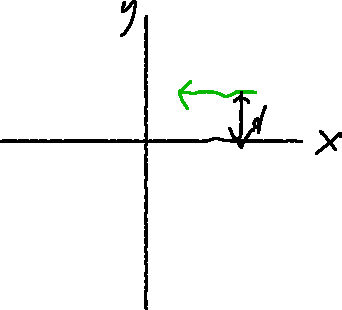
\includegraphics[width=6cm]{2-04-1.png}
	\caption*{The trajectory of light in our example}
\end{figure*}
\begin{align*}
	x &= r\cos\phi & y &= r\sin\phi \\
	b &= r^2 u^\phi
\end{align*}
And we say approximately:
\begin{align*}
	\phi &\approx \frac{d}{r} & \frac{dr}{dt} &= -1 & \frac{d\phi}{dt} &= \frac{d}{r^2}
\end{align*}


For timelike geodesics in the Schwartzchild geometry we have been heavilly relying on:
\begin{align*}
	\varepsilon &= \frac{1}{2}\left(\frac{dr}{d\tau}\right)^2 + V_\text{eff}(r) \\
	V_\text{eff}(r) &= -\frac{M}{r} + \frac{l}{2r^2} - \frac{Ml^3}{r^3} \\
	l &= r^2\sin^2\theta \frac{d\phi}{d\tau}
\end{align*}
We now look at:
\begin{align*}
	\frac{d\phi}{dr} &= \frac{\dot{\phi}}{\dot{r}} \\
	\frac{d\phi}{dr} &= \pm \frac{l}{r^2} \frac{1}{\sqrt{2(2-V_\text{eff}(r))}} \\
	\frac{d\phi}{dr} &= \pm \frac{l}{r^2} \left(e^2 - \left(1-\frac{2M}{r}\right)\left(1+ \frac{l^2}{r^2}\right)\right)^{-\frac{1}{2}}
\end{align*}
This allows us to look at our precession in terms of $\delta \phi = \Delta\phi -2\pi$:
\begin{align*}
	\Delta\phi &= 2l \int_{r_1}^{r_2} \frac{dr}{r^2}\left(e^2 - \left(1-\frac{2M}{r}\right)\left(1+ \frac{l^2}{r^2}\right)\right)^{-\frac{1}{2}}
\end{align*}
Although we could numerically evaluate it, it's interesting to consider what happens if we take a specific limit of this, so we can find that to leading order:
\begin{align*}
	\delta\phi &= 6\pi\left(\frac{GM}{cl}\right)^2 & l^2 &= GMa(1-\epsilon^2) \\
	\delta\phi &= \frac{6\pi G}{c^2} \frac{M}{a(1-\epsilon^2}
\end{align*}
And experimentally this is most relevant for the precession of Mercury.
\subsection{Deflection of light}
Working in the equitorial plane with light we can see:
\begin{align*}
	l&= r^2\frac{d\phi}{d\lambda} \\
	\frac{d\phi}{d\lambda} &= \frac{l}{r^2} \\
	\frac{1}{b^2} &= \frac{1}{l^2} \left(\frac{dr}{d\lambda}\right)^2 + W_\text{eff} \\
	\frac{dr}{d\lambda} &= \pm l \sqrt{\frac{1}{b^2} - W_\text{eff}} \\
	\frac{d\phi}{dr} &= \pm \frac{1}{r^2\sqrt{\frac{1}{b^2} - W_\text{eff}}}
\end{align*}
\begin{figure*}[h]
	\centering
	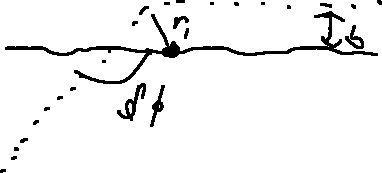
\includegraphics[width=6cm]{2-06-1.png}
	\caption*{Deflection of light}
\end{figure*}

We can then see:
\begin{align*}
	\Delta \phi &= 2\int_{r_1}^\infty \frac{dr}{r^2\sqrt{\frac{1}{b^2} - W_\text{eff}}}
\end{align*}
At our turning point $\frac{1}{b^2} = W_\text{eff}$, we can do a change of variables $r= \frac{b}{w}$:
\begin{align*}
	\Delta \phi &= 2\int_{0}^{w_1} \frac{dw}{\sqrt{1 - w^2\left(1- \frac{2M}{b}w\right)}}
\end{align*}
We can evaluate our value of $b$ which should be approximately the radius of the sun, and clearly $M$ is just the mass of the sun, so we find $\frac{2M}{b} \approx 10^{-6}$.
Therefore we should be find to expand in terms of $\frac{2M}{b}$:
\begin{align*}
	\Delta \phi &= 2\int_{0}^{w_1} \frac{dw}{\sqrt{1- \frac{2M}{b}w}\sqrt{\left(1- \frac{2M}{b}w\right)^{-1} - w^2}} \\
	\Delta \phi &= 2\int_{0}^{w_1} \frac{dw(1+ \frac{Mw}{b})}{\sqrt{1+ \frac{2M}{b}w - w^2}} \\
	\Delta \phi &= \pi + \frac{4M}{b} \\
	\delta\phi &= \delta\phi - \pi \\
	\delta\phi &= \frac{4GM}{c^2b}
\end{align*}
Which for the sun we see $\delta\phi \approx 1.7"$. This provides a measurable difference in the path that light takes.

Additionally we can see that we see a time delay for the passage of light compared to flat spacetime. 
We construct this in terms of a ranging experiment.
\begin{figure*}[h]
	\centering
	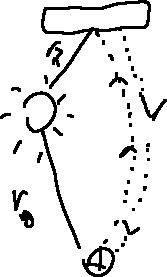
\includegraphics[width=4cm]{2-06-2.png}
	\caption*{Ranging experiment}
\end{figure*}

We see:
\begin{align*}
	e&= \left(1- \frac{2M}{r}\right)\frac{dt}{d\lambda} \\
	\frac{dt}{d\lambda} &= \left(1 - \frac{2M}{r}\right)^{-1} e \\
	\frac{dt}{dr} &= \pm \frac{1}{b}\left(1-\frac{2M}{r}\right)^{-1} \left[ \frac{1}{b^2} - W_\text{eff}\right]^{-\frac{1}{2}}
\end{align*}
And:
\begin{align*}
	\Delta t &= 2t(r_\oplus,r_1) + 2t(r_r,r_1) \\
	t(r,r_1) &=\int_{r_1}^r \frac{dr}{b}\left(1-\frac{2M}{r}\right)^{-1} \left[ \frac{1}{b^2} - W_\text{eff}\right]^{-\frac{1}{2}}
\end{align*}
We look only to first order in $M$ so we see:
\begin{align*}
	b &= r_1\left(1 - \frac{2M}{r_1}\right)^{-\frac{1}{2}} \\
	b &\approx r_1 + M
\end{align*}
So then we can see:
\begin{align*}
	t(r,r_1) &= \sqrt{r^2 - r_1^2} + 2M \log\frac{r+ \sqrt{r^2 - r_1^2}}{r_1} + M \frac{r-r_1}{r+r_1}
\end{align*}
Where the classical time is clearly $\sqrt{r^2 - r_1^2}$. So our excess time is then:
\begin{align*}
	\Delta t_\text{excess} &= \Delta t - 2\sqrt{r_\oplus^2 - r_1^2} - 2\sqrt{r_R^2  -r_1^2} \\
	\Delta t_\text{excess} &\approx \frac{4GM}{c^3} \left[\log\left(\frac{4r_Rr_\oplus}{r_1^2}\right) + 1\right]
\end{align*}
We call this the Shapiro time delay.

This time delay is important for binary star systems with pulsars and neutron stars.

\subsection{Paramaterized post-newtonian(PPN) framework}
We start with a generalized static spherically symmetric line element:
\begin{align*}
	ds^2 -A(r)dt^2 + B(r) dr^2 + r^2(d\theta^2 + \sin^2\theta d\phi^2)
\end{align*}
Where in these functions $A$ and $B$ we have a systematic way to introduce curvature from mass. In order to compare to Newtonian mechanics we do expansions in $\frac{1}{c}$ that give us Newtonian mechanics plus a correction term.
We assume that $M$ is the only parameter that influences our spacetime, so our expansion must be in terms of $\frac{GM}{c^2 r}$.
\begin{align*}
	A(r) &= 1 - \frac{2GM}{Pc^2 r} + \ldots \\
	B(r) &= 1 + \ldots
\end{align*}
We introduce parameters:
\begin{align*}
	A(r) &= 1 - \frac{2GM}{c^2 r} + 2(\beta - \gamma)\left(\frac{GM}{c^2 r}\right)^2  + \ldots \\
	B(r) &= 1 + 2\gamma \frac{GM}{c^2 r} + \ldots
\end{align*}
Where we will recover GR if $\gamma = \beta = 1$. We can think of this as $\gamma$ controlling how much space curvature ($g_{ij}$) is produced by a unit rest mass, and $\beta$ determines how much non-linearity there is in the superposition law for gravity ($g_{00}$).
We can alos introduce a $\beta_1$ that controls how much gravity is produced by unit kinetic energy and a $\beta_2$ which controls how much gravity is produced by unit gravitational potential energy, etc.
The convention is that GR is recovered when all parameters are equal to $1$.

We have constrained these experimentally to be:
\begin{align*}
	|\gamma-1| &\leq 2.3\time 10^{-5} \\
	|\beta - 1| &\leq 8\time 10^{-5}
\end{align*}


We now turn our attention to the anomalous perigelion advance of Mercury. Our total observed precession of Merecuries perihelion is $\delta\phi = 5599.74" \pm 0.41"$ per century. We can account for $532.3035"$ per century from other planets in the solar system.
Although there are other things that impact this, the dominant contribution is from the non-inertial frame we are observing from on earth. Once everything is taken into account we find that there are $42.9799"$ per century explained only by generally relativistic effects.

We now look at the experimental predictions of these theories:
\begin{align*}
	\delta\phi &= \left(\frac{1+\gamma}{2}\right)\left(\frac{4GM}{c^2 b}\right) & \text{Deflection of light}\\
	\delta\phi &= \frac{1}{3}(2+ 2\gamma-\beta) \frac{6\pi GM}{c^2a(1-\epsilon^2)} & \text{Perihelion precession} \\
	\Delta t &= \left(\frac{1+\gamma}{2}\right) \frac{4GM}{c^3} \left[ \ln \frac{4r_\oplus r_R}{r_1^2} + 1\right] & \text{Time delay of light}
\end{align*}
In 1974/1975 NRAO measured the deflection of radio signals from quasars of $\gamma = 1.007 \pm 0.009$.
As far as delay measurements go, we measured the delay of radio signals traveling from earth to mars of $\gamma = 1.000 \pm 0.002$.
For perihelion advances we found $\beta = 1.000 \pm 0.003$.

Looking at a description of gravitational lensing we can say that all our involved angles will typically be quite small. We know:
\begin{figure*}[h]
	\centering
	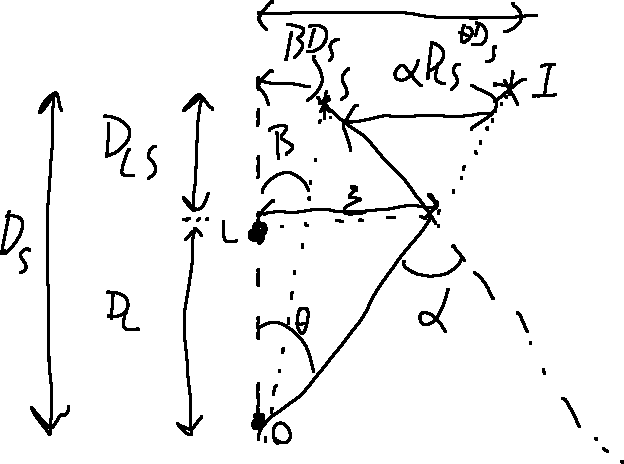
\includegraphics[width=8cm]{2-11-1.png}
	\caption*{Gravitational lensing}
\end{figure*}
\begin{align*}
	\alpha &= \frac{2R_s}{b}
\end{align*}
Where $R_s$ is the Schwartzchild radius of the lens. We know that $R_s \ll D_L,D_S,D_{LS}$. We can see we can derive the lens equation:
\begin{align*}
	\theta D_s &= \beta D_s + \alpha D_{LS}
\end{align*}
Where we can see $b\approx \xi$ and $\xi \approx \theta D_L$ So we can then say:
\begin{align*}
	\theta &= \beta + \frac{\theta_E^2}{\theta} &
	\theta_E &= \sqrt{2R_s \frac{D_{LS}}{D_S D_L}}
\end{align*}
Where we call $\theta_E$ the einstein angle.

With this in hand we now consider the lensing of a galactic star being lensed by anothe solar mass object, which gives us:
\begin{align*}
	R_s &\approx 1km & D_L &\approx 10^7 km \\
	\theta_E &\approx 10^{-3}"
\end{align*}

We now look at lensed versus unlensed images:
\begin{figure*}[h]
	\centering
	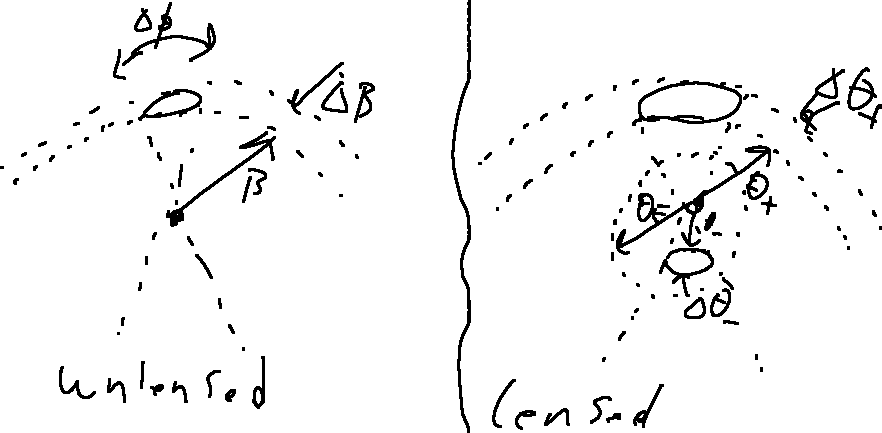
\includegraphics[width=12cm]{2-11-2.png}
	\caption*{Lensed vs. unlensed images}
\end{figure*}
\begin{align*}
	\theta &= \beta + \frac{\theta_E^2}{\theta} \\
	\theta^2 &= \beta\theta + \theta_E^2 \\
	\theta_\pm &= \frac{1}{2}\left[\beta\pm\sqrt{\beta^2 + 4\theta_E^2}\right]
\end{align*}
If we then differntiate this
\begin{align*}
	\Delta\theta_\pm &= \frac{1}{2}\left[1\pm\frac{\beta}{\sqrt{\beta^2 + 4\theta_E^2}}\right]
\end{align*}
If we now consider our brightness:
\begin{align*}
	\frac{I_\pm}{I_*} &= \frac{\Delta\Omega_\pm}{\Delta\Omega_*} \\
	\frac{I_\pm}{I_*} &= |\frac{\theta_\pm \Delta\theta_\pm}{\beta\Delta\beta}| \\
	\frac{I_\pm}{I_*} &= |\frac{\theta_\pm}{\beta} \frac{d\theta_\pm}{d\beta}| \\
	\frac{I_\pm}{I_*} &= \frac{1}{4}\left(\frac{\beta}{\sqrt{\beta^2 + 4\theta_E^2}} + \frac{\sqrt{\beta^2 + 4\theta_E^2}}{\beta} \pm 2\right)
\end{align*}
In the microlensing picture we see:
\begin{align*}
	\frac{I_\text{tot}}{I_*} &= \frac{I_+ + I_-}{I_*} \\
	\frac{I_\text{tot}}{I_*} &= \frac{1}{2}\left(\frac{\beta}{\sqrt{\beta^2 + 4\theta_E^2}} + \frac{\sqrt{\beta^2 + 4\theta_E^2}}{\beta}\right)
\end{align*}
We now consider a massive compact object in the halo of our galaxy. This could be something like a MACHO lensing a star in the LMC.
$\theta_E$ will be related to the mass of the MACHO, and $\beta$ will be changing in time as the MACHO moves.
The characteristic time here will be given by the time it takes our MACHO to traverse our charactoristic angular distance $\theta_E$.
We know:
\begin{align*}
	\theta_E &\approx 10^{-3} "& D_L &\approx 10 kpc & v &\approx 200 \frac{km}{s} \\
	t_\text{var} &= \frac{\theta_e D_L}{v} \\
	t_\text{var} &\approx 0.2 yr
\end{align*}

\subsection{Eddington-Finkelstein coordinates}
We now want to look at the Schwarztchild solution in terms of the physical system, instead of purely looking at the geometry.
Looking at the spacetime outside a collapsing star we want to consider what happens to the metric. It turns out that the ``Gauss's'' law picture of only the enclosed mass mattering happens to be correct in the generally relativistic picture.
In order to understand this we introduce a new set of coordinates:
\begin{align*}
	t &= v-r -2M \ln |\frac{r}{2M}  -1|
\end{align*}
Which allows us to rewrite our metric:
\begin{align*}
	dt &= dv - dr- \ldots
\end{align*}
For $r>2M$ we can say $\ln |\frac{r}{2M} - 1| = \ln \left(\frac{r}{2M}  -1 \right)$, and for $r < 2M$ we have $\ln |\frac{r}{2M} - 1| = \ln\left(1 - \frac{r}{2M}\right)$, so:
\begin{align*}
	ds^2 &= -\left(1-\frac{2M}{r}\right) dv^2 + 2dv dr + r^2(d\theta^2 + \sin^2\theta d\phi^2)
\end{align*}
Which happens to function for both roots. It turns out that the singularity at $r=0$ survives, and it will always be present regardless of what coordinates we pick.

We look at light cones in these coordinates to better understand the physical system. If we consider radial light cones we have:
\begin{align*}
	0 &= -\left(1-\frac{2M}{r}\right) dv^2 + 2dvdr
\end{align*}
This gives us solutions with constant $v$ which correspond to ingoing radial light rays. We have an additional solution where:
\begin{align*}
	v - 2(r+2M\ln|\frac{r}{2M} -1|) &= \text{const}
\end{align*}
Which will clearly be our outgoing lightrays. For $r>2M$ this is outgoing in the usual sense, but inside the Schwartzchild radius the sign will flip and these will still be ingoing rays.

It will be convenient to define a new time coordinate:
\begin{align*}
	\tilde{t} &= v-r
\end{align*}
We can see then:
\begin{align*}
	\tilde{t} + r-2(r+ 2M \ln |\frac{r}{2M} - 1|) &= \text{const} \\
	\frac{\tilde{t}}{M} &= \text{const} - \frac{r}{M} + 4\ln |\frac{r}{2M} - 1|
\end{align*}


We know that our light rays will all go to zero for $r<2M$, at $r=2m$ ``outgoing'' rays become stationary, and beyond that they can go outwards.
Our horizon is a 3-D null surface with normal vector in the r direction, and a null distance on it. This surface is a one way surface in the same way as a lightcone in flat space (once you pass through it you can't pass back out).

If we take a slice where $v=\text{const}$, then:
\begin{align*}
	d\Sigma^2 &= (2M)^2(d\theta^2 + \sin^2\theta d\phi^2)
\end{align*}
Which is a sphere of radius $2M$, so the ``Area'' is $A=16\pi M^2$.

Looking at this in terms of polar coordinates in flat spacetime, we know $r=0$ is a timelike worldline, i.e. it denotes a place in space for all times.
Looking instead at our Schwarzchild geometry, inside the Schwarzchild radius, we see:
\begin{align*}
	ds^2 (dr=0) &= -\left(1 - \frac{2M}{r}\right) dv^2 r^2 (d\theta^2 + \sin^2\theta d\phi^2)
\end{align*}
Which is always positive, and thus indicates a spacelike surface. This indicates that $r$ seems to have taken on a role more similar to a moment in time than a place in space.
Intuitively this is because there is no way for a particle to remain stationary within the Schwarzchild radius.

\subsection{Collapsing Star}
If we look at our geodesic equations for radial infall (from an infinite distance):
\begin{align*}
	r(\tau) &= \left(\frac{3}{2}\right)^\frac{2}{3} (2M)^\frac{1}{3}(\tau_* - \tau)^\frac{2}{3} \\
	t &= t_* + 2K\left[ -\frac{2}{3}\left(\frac{r}{2M}\right)^\frac{3}{2} - 2\left(\frac{r}{2M}\right)^\frac{1}{2} + \ln \frac{\sqrt{\frac{r}{2M}} +1}{\sqrt{\frac{r}{2M}} -1}\right]
\end{align*}
If we set $\tau = 0$ when $r=0$, then:
\begin{align*}
	\frac{v}{2M} &= \frac{r}{2M} - \frac{2}{3} \left(\frac{r}{2M}\right)^\frac{3}{2} + 2\ln| 1 + \sqrt{\frac{r}{2M}}|
\end{align*}
\begin{figure*}[h]
	\centering
	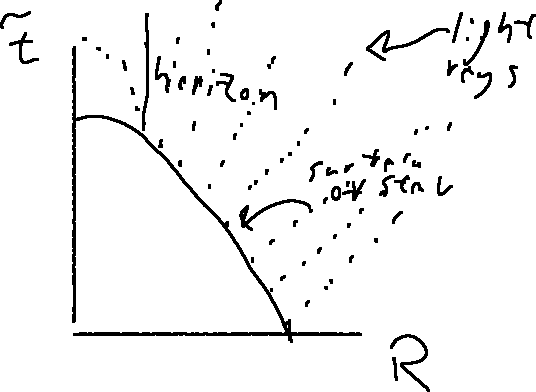
\includegraphics[width=12cm]{2-18-1.png}
	\caption*{Our collapsing star}
\end{figure*}
If we choose a proper time for our surface to go from $r=2m$ to $r0$. We say:
\begin{align*}
	r(\tau_H) &= 2M \\
	r(\tau_H) &=\left(\frac{3}{2}\right)^\frac{2}{3} (2M)^\frac{1}{3}(\tau_* - \tau_H)^\frac{2}{3} \\
	\tau_*^\frac{2}{3} &= 2M \left(\frac{3}{2}\right)^{-\frac{2}{r}} (2M)^{-\frac{1}{3}} \\
	\tau_* &= \frac{4M}{3} \\
	r(\tau_0) &= 0 \\
	0 &= \tau_* - \tau_0 \\
	\tau_0 &= \frac{4M}{3}
\end{align*}

\subsection{Redshifted light from collapsing star}
We now look at the redshift of the light coming from a collapsing star. We consider that the star emits light from the surface at fixed proper time intervals $\tau$, which is:
\begin{align*}
	\omega_* &= \frac{2\pi}{\tau}
\end{align*}
We look at what will be seen from a distant stationary observer. For this observer the proper and coordinate times are equivalent, so we look at time $t_R$ and consider the frequency the observer will observe $\omega_R(t_r) = \frac{2\pi}{\Delta t_R}$.

For ourgoing rays:
\begin{align*}
	v- 2\left(r + 2M \ln |\frac{r}{2M} -1 |\right) &= \text{const}
	v_E- 2\left(r_E + 2M \ln |\frac{r_E}{2M} -1 |\right) &= v_R- 2\left(r_R + 2M \ln |\frac{r_R}{2M} -1 |\right)
\end{align*}
Where $E$ denotes the emitter and $R$ denotes the reciever.

If we take the limit of a surface near the Schwarzchild horizon, and an extremely distant observer (and also using $t=v-r-2M\ln|\frac{r}{2M} - 1|$):
\begin{align*}
	- 4M \ln \left(\frac{r_E}{2M} -1 \right) &= t_R + r_R \\
	\frac{r_E}{2M}  -1 &= e^{-\frac{t_r - r_R}{4M}}
\end{align*}
Therefore the surface from which theobserver recieves light from, has an exponential with charactoristic time $4M$. So:
\begin{align*}
	\omega_R &= \frac{2\pi}{\Delta t_R} \\
	\omega_R &= \omega_* e^{-\frac{t_R}{4M}}
\end{align*}
Which will approach infinite redshifting with a timescale $4M$. This means that the black hole would immediately have all light become redshifting until it becomes undetectable, and therefore it suddenly appears dark.
\subsection{Kruskal coordinates}
Just like Eddington-Finkelstein coordinates, we trade our radial and temporal coordinates for new coordinates:
\begin{align*}
	U &= \sqrt{\frac{r}{2M} -1}e^{r}{4M} \cosh \frac{t}{4M} \\
	V &= \sqrt{\frac{r}{2M} - 1}e^{r}{4M} \sinh \frac{t}{4M}
\end{align*}
Outside the event horizon, and:
\begin{align*}
	U &= \sqrt{1-\frac{r}{2M}}e^{r}{4M} \sinh \frac{t}{4M} \\
	V &= \sqrt{1-\frac{r}{2M}}e^{r}{4M} \cosh \frac{t}{4M}
\end{align*}
Inside the even horizon, this gives us our line element:
\begin{align*}
	ds^2 &= \frac{32 M^3}{r} e^{-\frac{r}{2M}}(-dV^2 + dU^2) + r^2 (d\theta^2 + \sin^2\theta d\phi^2) \\
	\left(\frac{r}{2M} -1\right)e^\frac{r}{2M} &= U^2 -V^2
\end{align*}
So for lines of constant $r$ we have constant $U^2 - V^2$ and for constant $t$ we have:
\begin{align*}
	\tanh\frac{r}{4M} &= \frac{V}{U} & r &> 2M \\
	\tanh\frac{r}{4M} &= \frac{U}{V} & r &< 2M \\
\end{align*}
We say radial light rays obey:
\begin{align*}
	0 &= \frac{32 M^3}{r} e^{-\frac{r}{2M}}(-dV^2 + dU^2) \\
	V &= \pm U + \text{const}
\end{align*}
\begin{figure*}[h]
	\centering
	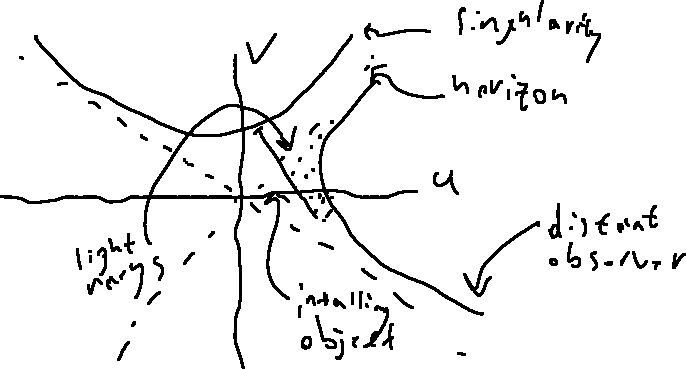
\includegraphics[width=12cm]{2-18-2.png}
	\caption*{Kruskal coordinates}
\end{figure*}
\subsection{Hand waving Hawking radiation}
Detailed calculations are outside the scope of this course, but we will look at relevant constants and come up with an argument for Hawking radiation.
If we consider the energy carried away by particles generated near the horizon then we consider the energy the black hole must lose to obey conservation of energy.
If we give our particle $\bm{p}$ four momentum, and it's pair particle $\tilde{\bm{p}}$ four momentum. If we consider the energy conservation driven by $\xi$ we see:
\begin{align*}
	\bm{\xi}\cdot\bm{p} + \bm{\xi}\cdot\tilde{\bm{p}} &= 0 \\
	\bm{\xi}\cdot\bm{\xi} &= 1 -\frac{2M}{r}
\end{align*}
So $\xi$ is timelike outside the horizon and spacelike inside it. Outside the horizen we have $-\bm{xi}\cdot\bm{p} >0$, which corresponds to the energy measured by an observer with a 4-velocity parrallel to our killing vector.
Inside the horizon $-\bm{\xi}\cdot\tilde{\bm{p}}$, this will become a momentum like term (because the role of the $t$ coordinate has flipped) and therefore it could be negative. We now look at the rate of change the black hole loses energy.
We start by saying that the rate should be proportional to $\hbar$, which has an associated length scale $l_p = \sqrt{\frac{G\hbar}{c^3}}$. We then say that this rate should look something like:
\begin{align*}
	\frac{dM}{dt} &= -\nu \frac{\hbar}{M^2}
\end{align*}
Where $\nu$ is a constant derived from QFT, but we find that this is going to be related to $\frac{\hbar}{8\pi M} = k_B T$
\begin{align*}
	M(t) &= \left[3\nu\hbar(t_* -t)\right]^\frac{1}{3}
\end{align*}
Which gives us an evaporation time $\tau \approx \frac{1}{3\nu}\frac{M^3}{\hbar}$ which is approximately $8.3 \times 10^{-26} \left(\frac{M}{1 g}\right)^3 s$
\section{Rotation}
When we say we are looking at slow rotation, we mean that our corrections should be only first order in angular velocity. Centripital accelerations then includes second order corrections.

This will allow us to see that the motion of this mass will change the curvature of the space. We call these gravito-magnetic effects.
\subsection{Slow Rotation in Schwarzchild geometry}
We consider test gyroscopes in order to probe spacetime. We can see our geodesics give us:
\begin{align*}
	\frac{d u^\alpha}{d\tau} &= -\Gamma_{\beta\gamma}^\alpha u^\beta u^\gamma
\end{align*}
In addition to our four velocity we also give our test gyroscope a spin vector, which is a spacelike vector $\bm{S}$. In a local inertial frame we can say:
\begin{align*}
	S^\alpha &= (0,\bm{S}) \\
	S_\alpha u^\alpha &= 0
\end{align*}
And our total spin is a constant of motion. In flat spacetime we should have:
\begin{align*}
	\frac{dS^\alpha}{d\tau} &= 0
\end{align*}
While in general we want it to obey everything we just said in local inertial components. We also want it to be linear in the components of our spin, and maintain the same form in all coordinate systems. Therefore we find:
\begin{align*}
	\frac{dS^\alpha}{d\tau} + \Gamma^\alpha_{\beta\gamma} S^\beta u^\gamma &= 0
\end{align*}


Our condition that $S_\alpha u^\alpha =0$ should hold in all frames.

We now turn our attention to the precession of a gryoscope moving in an orbit in Schwarzchild spacetime. We assume that our spin starts pointing along the $r$ direction. We can see that (working in the equatorial plane):
\begin{align*}
	S^\alpha u_\alpha &= -\left(1- \frac{2M}{r}\right) S^t u^ + R S^\phi u^\phi \\
	S^t &= \frac{R^2 S^\phi u^\phi}{u^t} \left(1 - \frac{2M}{r}\right)^{-1} \\
	S^t &=  R^2 \Omega\left(10\frac{2M}{r}\right)^{-1} S^\phi
\end{align*}
If we look at the radial component:
\begin{align*}
	\frac{dS^r}{d\tau} &= -\Gamma^r_{\beta\gamma} s^\beta u^\gamma \\
	\frac{dS^\phi}{d\tau} &= -\Gamma^\phi_{\beta\gamma} s^\beta u^\gamma \\
	\frac{dS^r}{dt}\frac{dt}{d\tau} + \Gamma^r_{tt} s^t u^t + \Gamma^r_{\phi\phi} S^\phi u^\phi &= 0 \\
	\frac{dS^r}{dt}u^t + \frac{M}{R^2}\left(1- \frac{2M}{r}\right) R^2 \Omega\left(1- \frac{2M}{r}\right)^{-1}  s^t u^t + (R-2M)\Omega S^\phi u^t &= 0 \\
	\frac{ds^r}{dt} - (R-3M)\Omega s^\phi &= 0 \\
	\frac{ds^\phi}{dt} + \frac{\Omega}{R} s^r &= 0 \\
	\frac{d^2 s^\phi}{dt^2} + \left(1-\frac{3M}{r}\right)\Omega^2s^\phi &= 0
\end{align*}
Which gives us a harmonic oscilator in $\phi$ with frequency $\Omega' = \sqrt{1 - \frac{3M}{r}}\Omega$ so:
\begin{align*}
	s^r &= S_* \sqrt{1-\frac{2M}{R}}\cos\Omega' t \\
	s^\phi &= -S_*\sqrt{1-\frac{2M}{R}}\frac{\Omega}{\Omega' R}\sin\Omega' t
\end{align*}
We then after one orbit we have:
\begin{align*}
	\frac{S^r}{S_*} &= \cos \frac{2\pi \Omega'}{\Omega} \\
	\frac{S^r}{S_*} &= \cos 2\pi\sqrt{1-\frac{3M}{R}} \\
	\Delta\phi &= 2\pi \left(1-\sqrt{1-\frac{3M}{R}}\right)
\end{align*}
For small $\frac{M}{R}$ we can say:
\begin{align*}
	\Delta\phi &\approx \frac{3\pi GM}{c^2 R}
\end{align*}
Which is approximately $8.4"$ per year for earth. This has been confirmed by experiment up to $0.5$.

\subsection{Outside a slowly rotating body}
We consider here only leading order effects from the rotation. We don't consider second order effects like changes to the spherical shape of our body.
GR wull predict changes to our metric entirely from the first order impact of the spinning object.
It can be shown that:
\begin{align*}
	ds^2 &= ds_\text{Schwartzchild}^2 - \frac{4G J}{c^3 r^2} \sin^2\theta (rd\phi)(cdt) + \mathcal{O}(J^2)
\end{align*}
We have our new quantity $\frac{GJ}{c^3 r^2}$ which governs the effects of the rotation. If we are rotating with angular speed $\Omega$ we have:
\begin{align*}
	J &\propto I\Omega \\
	J &\propto mR^2\Omega \\
	J &\propto mRV
\end{align*}
So:
\begin{align*}
	\frac{GJ}{c^3 r^2} &\propto \frac{GM}{c^2 R} \frac{V}{c}
\end{align*}
We now consider the case of a radially infalling gyroscope in this metric. We additionally choose for our gyroscope to fall along the axis of rotation of our central body.
Finally we choose the direction of the gyroscope to be perpendicular to the axis of rotation.
We want to find the precession rate to leading order in $\frac{1}{c}$, which happens to be a $\frac{1}{c^3}$ contribution.
If we work in cartesian coordinates:
\begin{align*}
	ds^2 &= ds_\text{Schwartzchild}^2 - \frac{4G J}{c^3 r^2} (cdt) \frac{xdy - ydx}{r} + \mathcal{O}(J^2)
\end{align*}
We use our equation for precession now:
\begin{align*}
	\frac{dS^\alpha}{d\tau} + \Gamma^\alpha_{\beta\gamma} S^\beta u^\gamma &= 0
\end{align*}
In the Schwartzchild geometry our fators of $\frac{GM}{Pc^2r}$ will become $\frac{GM}{c^2 r} \frac{GJ}{c^3 r^2}$, which we can then ignore as the correction is too small.
Therefore we consider:
\begin{align*}
	ds^2 &= ds_\text{flat}^2 - \frac{4GJ}{c^3 r^2} (cdt) \frac{xdy - ydx}{r}
\end{align*}
We have a four velocity that should simply be $u = (u^t,0,0,u^z)$ and $s = (0,S^x,S^y,0)$.
We now need to compute our Christofel symbols:
\begin{align*}
	g_{\alpha\delta} \Gamma^\delta_{\beta]gamma} &= \frac{1}{2} \left(\partder{g_{\alpha\beta}}{x^\gamma} + \partder{g_{\alpha\gamma}}{x^\beta} - \partder{g_{\beta\gamma}}{x^\alpha}\right)
\end{align*}
And we have metric elements:
\begin{align*}
	g_{tt} &= -c^2 & g_{xx} = g_{yy} = g_{zz} &= 1 \\
	g_{tx} &= \frac{2GJy}{c^2 z^3} & g_{ty} &= -\frac{2GJz}{c^2z^3}
\end{align*}
So then our only surviving derivitives become:
\begin{align*}
	\partder{g_{tx}}{y} &= \frac{2GJ}{c^2z^3} \\
	\partder{g_{ty}}{x} &= -\frac{2GJ}{c^2z^3}
\end{align*}
And some terms relating to $z$ which we will here ignore calculating since they don't appear in our computations. We can see:
\begin{align*}
	g_{tt}\Gamma^t_{\beta\gamma} + g_{tx} \Gamma^x_{\beta\gamma} + g_{ty} \Gamma^y_{\beta\gamma} + g_{tz} \Gamma^z_{\beta\gamma} &= -c^2\Gamma^t_{\beta\gamma}
\end{align*}
Because we are looking at paths where $x=y=0$L
\begin{align*}
	\Gamma^t_{\beta\gamma} &= 0
\end{align*}
And:
\begin{align*}
	g_{xt}\Gamma^t_{\beta\gamma} + g_{xx}\Gamma^x_{\beta\gamma} + \ldots &= \Gamma^x_{\beta\gamma}
\end{align*}
So:
\begin{align*}
	\Gamma^x_{\beta\gamma} &= \frac{1}{2}\left(\partder{g_{x\beta}}{x^\gamma} + \partder{g_{x\gamma}}{x^\beta} - \partder{g_{\beta\gamma}}{x}\right)
\end{align*}
If $\beta = t$ we can say:
\begin{align*}
	\Gamma^x_{ty} &= \frac{2GJ}{c^2z^3} & \Gamma^y_{tx} &= -\frac{2GJ}{c^2z^3}
\end{align*}
So:
\begin{align*}
	\frac{dS^x}{dt} &= -\frac{2GJ}{c^2z^3}S^y & \frac{dS^y}{dt} &= \frac{2GJ}{c^2z^3} S^x
\end{align*}


\section{Rotating Black Holes (Kerr Geometry)}
The black hole can be described by a dimensionless quantity representing the spin $a = \frac{J}{M}$, a parameter $\rho^2 = r^2 + a^2 \cos^2\theta$ and $\Delta = r^2 - 2Mr + a^2$. 
Our metric will be:
\begin{align*}
	ds^2 &= -\left(1-\frac{2Mr}{\rho^2}\right)dt^2 - \frac{4Mar\sin^2\theta}{\rho^2} d\phi dt + \rho^2 d\theta^2 + \left(r^2 + a^2 + \frac{2Mra^2\sin^2\theta}{\rho^2}\right)\sin^2\theta d\phi^2 + \frac{\rho^2}{\Delta} dr^2
\end{align*}
Clearly in the limit where $r \gg M$ we see we have flat space time. If instead we consider $r\gg a$ then:
\begin{align*}
	ds^2 &= -\left(1-\frac{2Mr}{r^2}\right)dt^2 + \rho^2 d\theta^2 + \left(1 + \frac{2M}{r}\right) dr^2 + r^2 (d\theta^2 + \sin^2\theta d\phi^2) - \frac{4Ma}{r^2} \sin^2\theta (rd\phi) dt
\end{align*}
Which is the expansion we found for a slowly rotating body

We can see that our metric is time independant, and $\phi$ independant, so we get two killing vectors:
\begin{align*}
	\xi^\alpha &= (1,0,0,0) \\
	\eta^\alpha &= (0,0,0,1)
\end{align*}

This has singularities when $\rho = 0$ or $\Delta = 0$. Clearly $\Delta = 0 \to r_\pm M \pm \sqrt{M^2 -a^2}$ where we assume $a < M$. Looking at the limit where $a=0$ we can see that $r_+$ corresponds the Schwarzchild radius.
For any black hole we have $a<M$ so we can argue that not only will black holes only form with less than this much angular momentum, but they can't absorb angular momentum that would put them over this limit.

\subsection{The Horizon}
We recall horizons are null surfaces identified by light rays remaining on the surface for all time.

If we tak  a surface of constant radius, looking at tangent vectors to this surface we can see:
\begin{align*}
	t^\alpha &= (t^t,0,t^\theta,t^\phi)
\end{align*}
We can also say our surface is null if at all points one null tangent vetor $\bm{l}$ can be found with two orthogonal spacelike tangent vectors. Therefore:
\begin{align*}
	\bm{l}\cdot\bm{l} &= g_{tt} (l^t)^2 + 2 g_{t\phi} l^tl^\phi + g_{\phi\phi} (l^\phi)^2 + g_{\theta\theta} (l^\theta)^2\\
	0 &= g_{tt} (l^t)^2 + 2 g_{t\phi} l^tl^\phi + g_{\phi\phi} (l^\phi)^2  + g_{\theta\theta} (l^\theta)^2\\
	0 &= \left(\frac{2Mr_+\sin\theta}{\rho_+}\right)^2 \left(l^\phi - \frac{a}{2Mr_+} l^t\right)^2 + \rho_+^2(l^\theta)^2
\end{align*}
Our general solution is that $l^\theta = 0$ and $l^\phi - \frac{a}{2Mr_+} l^t$. So we can say:
\begin{align*}
	l^\alpha &= (1,0,0,\Omega_H) & \Omega_H &= \frac{a}{2Mr_+}
\end{align*}
We can see by inspection that we have two spacelike tangent vectors $\hat{e}_r$ and $\hat{e}_\theta$. This shows that the photons on the event horizon rotate with the black hole.

For light rays moving along $\bm{l}$ we can say:
\begin{align*}
	\frac{d\phi}{d\lambda} &= \Omega_H
\end{align*}
If we look a the geometry at the horizon, setting $r=r_+$ and $t=\text{const}$ we can say:
\begin{align*}
	d\Sigma^2 &= \rho_+^2d\theta^2 + \left( r_+^2 + a^2 + \frac{2Mr_+ a^2\sin^2\theta}{\rho_+^2}\right)\sin^2\theta d\phi^2 \\
	d\Sigma^2 &= \rho_+^2d\theta^2 + \left(\frac{2Mr_+}{\rho_+}\right)^2\sin^2\theta d\phi^2 
\end{align*}
Which is not a spherical geometry, we can see that the distance around the equator is $4\pi M$ while around the poles it is $7.6 M$.

If we see that our area is then:
\begin{align*}
	A &= 8\pi M r_+ \\
	A &= 8\pi M (M + \sqrt{M^2 -a^2})
\end{align*}
\subsection{Orbits}
From our killing vectors we can see that we have conserved energy and conserved $z$ angular momentum.
Since we don't have conservation of angular momentum in general, we have no reason to expect a planar orbit, and will only see planar orbits if we have $\theta = \frac{\pi}{2}$.
For simplicity we consider these special planar orbits, to understand the effects on the radial motion.
Our metric is then:
\begin{align*}
	ds^2 &= -\left(1-\frac{2M}{r}\right)dt^2 - \frac{4Ma}{r} d\phi dt + \frac{r^2}{\Delta} dr^2 + \left(r^2 + a^2 + \frac{2Ma^2}{r}\right)d\phi^2
\end{align*}
We have constants of motion (for timelike trajectories):
\begin{align*}
	\bm{\xi}\cdot\bm{u} &= -e \\
	\bm{\eta}\cdot\bm{u} &= l \\
	\bm{u}\cdot\bm{u} &= -1
\end{align*}
So:
\begin{align*}
	-e &= g_{tt} u^t + g_{t\phi} u^\phi \\
	l &= g_{\phi t} u^t g_{\phi\phi} u^\phi \\
	u^t &= \frac{1}{\Delta}\left[\left(r^2 + a^2 + \frac{aMa^2}{r}\right)e - \frac{2Ma}{r} l\right] \\
	u^\phi &= \frac{1}{\Delta}\left[\left(1 - \frac{2M}{r}\right)l + \frac{2Ma}{r}e\right] \\
	\frac{e^2 - 1}{2} &= \frac{1}{2} \left(\frac{dr}{d\tau}\right)^2 + V_\text{eff}(r,e,l) \\
	V_\text{eff} &= -\frac{M}{r} + \frac{l^2 - a^2(e^2 -1)}{2r^2} - \frac{M(l-ae)^2}{r^3}
\end{align*}
Similarly for null trajectories we find:
\begin{align*}
	\frac{1}{l^2} \left(\frac{dr}{d\lambda}\right)^2 &= \frac{1}{b^2} - W_\text{eff}(r,b,\sigma) \\
	W_\text{eff}(r,b,\sigma) &= \frac{1}{r^2}\left[ 1- \frac{a^2}{b^2} - \frac{2M}{r}\left(1- \sigma \frac{a}{b}\right)^2\right] \\
	\sigma &= \text{sign}(l)
\end{align*}
\begin{figure*}[h]
	\centering
	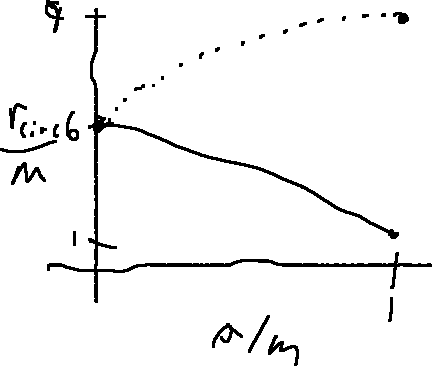
\includegraphics[width=12cm]{2-25-1.png}
	\caption*{The inner most stable radius for a circular orbit as a function of spin, the dotted lines are counter rotating}
\end{figure*}
For $a=M$ we see $e= \frac{1}{\sqrt{3}}$ $l = \frac{2M}{\sqrt{3}}$ and $r_\text{isco} = M$.
\subsection{Binding Energy}
The binding energy is the difference between the energy of a particle at rest at $\infty$ and the energy that the particle has moving in an orbit, as measured at infinity.

Since our rest mass energy is 1, we can say the binding energy per unit rest mass is $1-e$
\begin{figure*}[h]
	\centering
	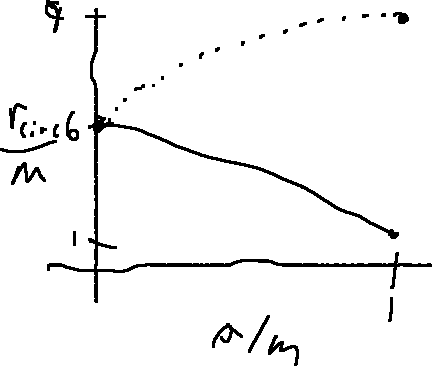
\includegraphics[width=12cm]{2-25-1.png}
	\caption*{Binding energy as a function of spin, the dotted line is counterrotating}
\end{figure*}
Clearly our corating ISCO is the ``most bound'' orbit, with this releasing $42\%$ of the rest mass energy of the particle when placed into this orbit.
\subsection{Ergosphere}
For the Schwartzchild geometry we can always remain a stationary observer as long as we are outside of the Schwarzchild radius. We want to consider what is needed to achieve this in the Kerr geometry (and whether or not it is even achievable).
To remain stationary we want:
\begin{align*}
	u^\alpha &= (u^t,0,0,0)
\end{align*}
And we know:
\begin{align*}
	-1 &= g_{tt} (u^t)^2 \\
	-1 &= -\left(1- \frac{2Mr}{\rho^2}\right) (u^t)^2 \\
\end{align*}
So this can only be satisfied when:
\begin{align*}
	r &> r_e & r_e &= M + \sqrt{M^2 - a\cos^2\theta}
\end{align*}
In order to avoid infall at a radius less that this new radius than we need to have our particle rotate along with the black hole.


\section{Differential Geometry}
\subsection{Vectors}
In order to look at vectors in a more general space we need to consider our vectors as something seperate from a line segment in flat space.
If we consider a function $f(x^\alpha)$ and a curve $x^\alpha(\sigma)$. The derivitive is therefore defined as:
\begin{align*}
	\frac{df}{d\sigma} &= \lim_{\epsilon\to0} \frac{f(x^\alpha(\sigma + \epsilon) - f(x^\alpha(\sigma)}{\epsilon} \\
	\frac{df}{d\sigma} &= \frac{dx^\alpha}{d\sigma} \partder{f}{x^\alpha}
\end{align*}
We then define our vector tangent to this curve $t^\alpha = \frac{dx^\alpha}{d\sigma}$. This mapping between directional derivatives and vectors is a 1-1 correspondance.
For any vector $a^\alpha$ corresponding to a directional derivitive we can write this as:
\begin{align*}
	\bm{a} &= a^\alpha \partder{}{x^\alpha}
\end{align*}
Where these partial derivitives now take the role of basis vectors. This correspondence between our basis vectors and our directional derivatives gives us a way of calculating basis transformations:
\begin{align*}
	\bm{a} &= a^\alpha \partder{x'\ ^\beta}{x^\alpha} \partder{}{x'\ ^\beta} \\
	a'\ ^\beta &= \partder{x'\ ^\beta}{x^\alpha} a^\alpha & a^\beta &= \partder{x^\beta}{x'\ ^\alpha} a'\ ^\alpha
\end{align*}

\subsection{Dual Vectors}
A dual vector is a linear map from vectors to real numbers. The real number that $\bm{\omega}$ maps $\bm{a}$ to is called $\omega(\bm{a})$. This should obey:
\begin{align*}
	\omega(\alpha \bm{a} + \beta\bm{b}) &= \alpha\omega(\bm{a}) \beta\omega(\bm{b})
\end{align*}
This can be represented as $\omega(\bm{a}) = \omega_\alpha a^\alpha$ clearly in order to obey all our linearity constraints. $\omega_\alpha$ are called the components of our dual vector.
We can say that the gradient of a function is a dual vector. If we recall that the derivitive of a function specifies a tangent vector $\bm{t}$, Then our gradient becomes:
\begin{align*}
	\partder{f}{x^\alpha}t^\alpha
\end{align*}
Where the $t^\alpha$ is a vector and $\partder{f}{x^\alpha}$ is our dual vector.

We can tell that clearly a set of four linearly independant dual vecotrs $\bm{e}^\alpha$ will provide a basis for all dual vectors:
\begin{align*}
	\bm{\omega} &= \omega_\alpha \bm{e}^\alpha
\end{align*}
Where these have been related to our normal basis vectors via:
\begin{align*}
	e^\alpha(\bm{e}_\beta) &= \delta^\alpha_\beta
\end{align*}

Putting this together we see:
\begin{align*}
	\omega(\bm{a}) &= \omega_\alpha e^\alpha(a^\beta\bm{e}_\beta) \\
	\omega(\bm{a}) &= \omega_\alpha a^\beta e^\alpha(\bm{e}_\beta) \\
	\omega(\bm{a}) &= \omega_\alpha a^\beta \delta_\beta^\alpha \\
	\omega(\bm{a}) &= \omega_\alpha a^\alpha
\end{align*}
\subsection{Correspondence between vectors and dual vectors}
Given a coordinate basis we can say:
\begin{align*}
	\bm{e}_\alpha(x)\cdot\bm{e}_\beta(x) &= g_{\alpha\beta}(x) \\
	\bm{a}\cdot\bm{b} &= g_{\alpha\beta} a^\alpha b^\beta
\end{align*}
So:
\begin{align*}
	a_\alpha &= g_{\alpha\beta}a^\beta
\end{align*}
We can then define an inverse metric such that:
\begin{align*}
	g_{\alpha\beta}g^{\beta\gamma} &= \delta_\alpha^\gamma \\
	a^\alpha &= g^{\alpha\beta}a_\beta
\end{align*}
If we have an orthonormal basis where $g_{\alpha\beta} = \eta_{\hat{\alpha}\hat{\beta}}$ then:
\begin{align*}
	a_{\hat{0}} &= - a^{\hat{0}} & a_{\hat{i}} &= a^{\hat{i}}
\end{align*}
We can use our basis vectors to project to components:
\begin{align*}
	\bm{e}^\alpha \cdot \bm{a} &= \bm{e}^\alpha\cdot a^\beta \bm{e}_\beta \\
	\bm{e}^\alpha \cdot \bm{a} &= a^\beta \bm{e}^\alpha\cdot \bm{e}_\beta \\
	\bm{e}^\alpha \cdot \bm{a} &= a^\beta \delta^\alpha_\beta \\
	\bm{e}^\alpha \cdot \bm{a} &= a^\alpha
\end{align*}
If we know the components $a^\alpha$ of a vector in a corrdinate bassis, then if we can say our coordinate basis components of orthonormal basis vectors and our dual basis are known then we can find our orthonormal components:
\begin{align*}
	a^{\hat{\alpha}} &= (e^{\hat{\alpha}})_\alpha a^\alpha & a_{\hat{\alpha}} &= (e_{\hat{\alpha}})^\alpha a_\alpha
\end{align*}

Taking as an example skew rectangular coordinates in flat space. In these coordinate $x$ and $y$ are not orthogonal and instead have an angle $\psi$ between them. We have a line element:
\begin{align*}
	dS^2 &= dx^2 + 2\cos\psi dxdy + dy^2
\end{align*}
We can see that clearly our dual basis vectors must be orthoogonal to the basis vectors they aren't associated with.
We can see that the lengths of the dual vectors can (and in general must) be non-unit in order to have our orthogonal relationships.
\begin{figure*}[h]
	\centering
	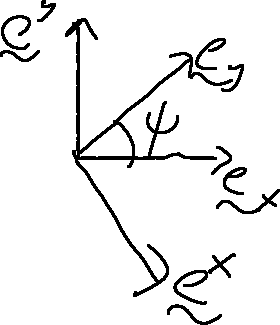
\includegraphics[width=12cm]{2-27-1.png}
	\caption*{Skew rectangular coordinates}
\end{figure*}

We now look at the example of normal vectors in 3-D space. Given a 3-surface in 4-D spacetime. 
We define the 3-surface in  terms of a function that is constrained, i.e. $f(x^\alpha) =\text{const}$. The gradient of $f$ will provide a normal vector:
\begin{align*}
	n_\alpha &= \partder{f}{x^\alpha}
\end{align*}
\subsection{Tensors}
We say that a vector is a bilinear (or more) map from pairs (or more) vectors into real numbers.

The metric is the tensor that maps two vectors into their inner product:
\begin{align*}
	g(\bm{a},\bm{b}) &= \bm{a}\cdot\bm{b}
\end{align*}
A rank r tensor is a r-linear map from r vectors to $\mathbb{R}$. We can write the tensor in terms of either the vector or dual vector basis. We can see:
\begin{align*}
	t(\bm{a},\bm{b},\bm{c}) &= t_{\alpha\beta\gamma} a^\alpha b^\beta c^\gamma \\
	t(\bm{a},\bm{b},\bm{c}) &= t_{\alpha\beta\gamma} a^\alpha b^\beta g^{\gamma\delta}c_\delta \\
	t(\bm{a},\bm{b},\bm{c}) &= t_{\alpha\beta}^{\ \ \gamma} a^\alpha b^\beta c_\gamma \\
	t_{\alpha\beta\gamma} &= t_{\alpha\beta}^{\ \ \delta}g_{\gamma\delta}
\end{align*}
And so on and so forth, we can change our representation to have any mix of upper and lower components using the metric.
We can also see that this gives us a mechanism to use tensors to map other tensors into other tensors, ex:
\begin{align*}
	v_\alpha &= t_{\alpha\beta\gamma} a^\beta b^\gamma
\end{align*}
If we sum upper and lower indicies, we call it a contraction (or sometimes a trace), ex:
\begin{align*}
	\omega_\alpha &= t_{\alpha\beta}^\beta
\end{align*}
Notably some objects that initially look like tensors (like Christoffel symbols) do not behave like tensors.
\subsection{Converting Tensor Components}
We want to look at converting our tensor components from coordinate basis to orthonormal basis.
We can describe any rank two tensor in terms of two vectors:
\begin{align*}
	t_{\alpha\beta} &= u_\alpha v_\beta
\end{align*}
We know that our orthonormal components can be calculated by:
\begin{align*}
	u_{\hat{\alpha}} &= (e_{\hat{\alpha}})^\alpha u_\alpha
\end{align*}
So:
\begin{align*}
	t_{\hat{\alpha}\hat{\beta}} &= (e_{\hat{\alpha}})^\alpha (e_{\hat{\beta}})^\beta u_\alpha v_\beta \\
	t_{\hat{\alpha}\hat{\beta}} &= (e_{\hat{\alpha}})^\alpha (e_{\hat{\beta}})^\beta t_{\alpha\beta}
\end{align*}

If we now look at going between different coordinate basis $x^\alpha$ and $x'\ ^\alpha$. Clearly we know:
\begin{align*}
	a_\alpha b^\alpha &= a'_\beta b'\ ^\beta \\
	a^\beta &= \partder{x^\beta}{x'\ ^\alpha}a'\ ^\alpha & a'_\beta &= \partder{x^\alpha}{x'\ ^\beta}a_\alpha
\end{align*}
And so we can write:
\begin{align*}
	g'_{\alpha\beta} &= \partder{x^\gamma}{x'\ ^\alpha} \partder{x^\delta}{x'\ ^\beta} g_{\gamma\delta} \\
	t'_\beta\ ^\alpha &= \partder{x'\ ^\alpha}{x^\gamma}\partder{x^\delta}{x'\ ^\beta} t^\gamma_\delta
\end{align*}
\subsection{Derivatives of vectors in curved space}
We have established that the partial derivitive of a function $f$ will give us a (dual) vector $\del f$ with components:
\begin{align*}
	(\del f)_\alpha &= \partder{f}{x^\alpha}
\end{align*}
We expect the derivative of our vector to be a rank 2 tensor as a result of the fact that this seems to be increasing the rank of the field. So $\del\bm{v} = \partial_\alpha v^\beta$.
This definition should involve the difference between vectors at nearby points in spactime. In order to make these comparisons we need a mechanism to transport vectors through spacetime.
This mechanism is known as parallel transport and we can define it in terms of:
\begin{align*}
	\del_t \bm{v}(x^\alpha) &= \lim_{\epsilon\to0} \frac{\bm{v}(x^\alpha + t^\alpha\epsilon)_\text{trans to $x^\alpha$} - \bm{v}(x^\alpha)}{\epsilon}
\end{align*}
\begin{figure*}[h]
	\centering
	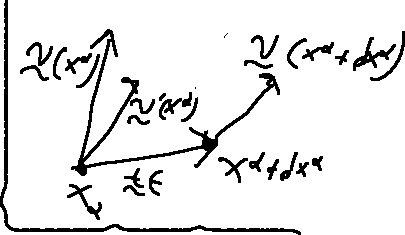
\includegraphics[width=12cm]{2-27-2.png}
	\caption*{Parallel transport}
\end{figure*}


\end{document}
